\documentclass[12pt,english,brazil,a4paper,utf8,oneside]{utfpr-tcc}

%Reviewing
\newcommand{\filipe}[1]{\textcolor{blue}{{\it [Filipe: #1]}}}
% copying from you, Filipe, hahaa
\newcommand{\daniel}[1]{\textcolor{red}{{\it [Daniel: #1]}}}

% carrega o arquivo configuracoes.tex que contém os pacotes e comandos Latex.
%
% Esse arquivo conterá pacotes e comandos utilizados na monografia
%
% Observação - devido a um erro do sharelatex foi necessário colocar na raiz do projeto os seguintes arquivos:
% gcnumparser.sty, fcprefix.sty, fmtcount.sty, fc-poruges.def, fcportuguese.def.
% Tal problema foi relatado em: https://github.com/nlct/fmtcount/issues/26
% Quando o sharelatex corrigir o problema acredito que podemos remover esses arquivos do projeto. At. Luiz Arthur.
%

% Este comando não é necessário: utilizei apenas para deixar o latex2rtf
% feliz (e descobrir a codificação do texto).
\usepackage[utf8]{inputenc}

% Suporte a figuras e subfiguras
\usepackage{graphics}
\usepackage{subfigure}

% Suporte a tabelas (principalmente do cronograma)
\usepackage{tabularx}
\usepackage{multirow}
\usepackage{array}
\usepackage{tabularx}
\usepackage{colortbl}
\usepackage{hhline}
\usepackage{xcolor}


% better tables
\usepackage{booktabs}

% frame box
\usepackage{mdframed}

% Escalar fontes para redimencionar, por exemplo tabelas
\usepackage{scalefnt}

% Algoritmos.
\usepackage{algorithm,algorithmic}

\usepackage[alf]{abntex2cite}

% the table's styles
\usepackage{booktabs}

% Elementos geralmente utilizados na tabela do cronograma
\newcommand{\fullcell}{\multicolumn{1}{>{\columncolor[gray]{0.5}}c}{}}
\newcommand{\fullcellline}{\multicolumn{1}{>{\columncolor[gray]{0.5}}c|}{}}
\newcommand{\mc}[3]{\multicolumn{#1}{#2}{#3}}
\newcommand{\y}{\rule{8pt}{4pt}}
\newcommand{\n}{\hspace*{8pt}}

% Define o caminho das figuras
\graphicspath{{images/}}

%% Configuração de glossário
\usepackage[portuguese]{nomencl}
\usepackage[nogroupskip,acronym,nomain,nonumberlist,nopostdot,nohypertypes={acronym}]{glossaries}

\makenoidxglossaries

% para siglas em português
\newcommand{\sigla}[2]
{
 \newglossaryentry{#1}{
  name=#1,
  description={#2},
  first={#2 (#1)},
  long={#2}
 }  
}

% para siglas de língua estrangeira, nessas a descrição longa fica em itálico.
\newcommand{\siglaIt}[2]
{
 \newglossaryentry{#1}{
  name=#1,
  description={\textit{#2}},
  first={\textit{#2} ({#1})},
  long={\textit{#2}}
 }  
}

% --- Estilos para apresentação de Código ----- %
\usepackage{listings}
\lstset{escapechar=§}
\lstloadaspects{formats}

\lstset{
	aboveskip=0cm,
	stringstyle=\ttfamily,
	showstringspaces = false,
	basicstyle=\scriptsize\ttfamily,
	commentstyle=\color{gray!45},
	keywordstyle=\bfseries,
	ndkeywordstyle=\bfseries,
	identifierstyle=\ttfamily,
	numbers=left,
	numbersep=15pt,
	numberstyle=\tiny,
	numberfirstline = false,
	breaklines=true
}

\lstdefinelanguage{JavaScript}{
	keywords={typeof, new, true, false, catch, function, return, null, catch, switch, var, const, let, async, await, if, in, while, do, else, case, break, from},
	ndkeywords={class, export, boolean, throw, implements, import, this},
	sensitive=false,
	comment=[l]{//},
	morecomment=[s]{/*}{*/},
	morestring=[b]',
	morestring=[b]"
}

% Diff language
\usepackage{xcolor}
\definecolor{diffstart}{named}{lightgray}
\definecolor{diffincl}{named}{blue}
\definecolor{diffrem}{named}{red}

\lstset{
	aboveskip=0cm,
	stringstyle=\scriptsize,
	showstringspaces = false,
	basicstyle=\scriptsize\ttfamily,
	commentstyle=\color{gray!45},
	keywordstyle=\bfseries,
	ndkeywordstyle=\bfseries,
	identifierstyle=\ttfamily,
	numbers=left,
	numbersep=15pt,
	numberstyle=\tiny,
	numberfirstline = false,
	breaklines=true
}

\lstdefinelanguage{diff}{
    basicstyle=\scriptsize\ttfamily,
	morecomment=[f][\color{diffstart}]{@@},
	morecomment=[f][\color{diffincl}]{+\ },
	morecomment=[f][\color{diffrem}]{-\ },
	morestring=[b]',
	morestring=[b]",
	keywords={typeof, new, true, false, catch, function, return, null, catch, switch, var, const, let, async, await, if, in, while, do, else, case, break, from},		
	ndkeywords={class, export, boolean, throw, implements, import, this},
}
% --- Fim da Definição de Estilos para apresentação de Código ----- %
% carrega o arquivo constantes.tex que contém dados do curso/monografia que NÃO DEVEM ser alterados. 
% Dados do curso que não precisam de alteração
\university{Universidade Tecnológica Federal do Paraná}
\universityen{Federal University of Technology -- Paraná}
\universityunit{Departamento Acadêmico de Computação}
\address{Campo Mourão}
\addressen{Campo Mourão, PR, Brazil}
\documenttype{Monografia}
\documenttypeen{Monograph}
\degreetype{Graduação}
% carrega o arquivo variaveis.tex que contém dados do acadêmico/monografia que DEVEM ser alterados.
% Dados do curso. Caso seja BCC:
\program{Curso de Bacharelado em Ciência da Computação}
\programen{Undergradute Program in Computer Science}
\degree{Bacharel}
\degreearea{Ciência da Computação}
% Caso seja TSI:
% \program{Curso Superior de Tecnologia em Sistemas para Internet}
% \programen{Undergradute Program in Tecnology for Internet Systems}
% \degree{Tecnólogo}
% \degreearea{Tecnologia em Sistemas para Internet}


% Dados da disciplina. Escolha uma das opções e a descomente:
% TCC1:
\goal{Proposta de Trabalho de Conclusão de Curso de Graduação}
\course{Trabalho de Conclusão de Curso 1}
% TCC2:
% \goal{Trabalho de Conclusão de Curso de graduação}
% \course{Trabalho de Conclusão de Curso 2}


% Dados do TCC (precisa alterar)
\author{Daniel Venturini}  % Seu nome
\title{Estudo empírico sobre \textit{Break change} no ecossistema do NPM} % Título do trabalho
\titleen{An Empirical Study of Breaking Changes in the npm Ecosystem } % Título traduzido para inglês
\advisor{Prof. Dr. Ivanilton Polato} % Nome do orientador. Lembre-se de prefixar com "Prof. Dr.", "Profª. Drª.", "Prof. Me." ou "Profª. Me."}
\coadvisor{Prof. Dr. Igor Scaliante Wiese} % Nome do coorientador, caso exista. Caso não exista, comente a linha.
\depositshortdate{2019} % Ano em que depositou este documento

% Dados da ficha catalografica. Ela é opcional, mas é uma boa ideia inserí-la. Exemplos para geração (http://fichacatalografica.sibi.ufrj.br/)
\fichacatautor{}  % Nome conforme citado (ou seja, no formato "Sobrenome, Nome").
\fichacatbib{Biblioteca da UTFPR de Campo Mourão} % Não alterar
\fichacatpum{M488} % Código Cutter-Sanborn. Use a primeira letra do sobrenome seguido do número conforme as primeiras letras do sobrenome e a tabela http://www.amormino.com.br/cutter-sanborn/cutter1.html
\fichacatpalcha{} % Assuntos do trabalho. Cada item deve ser enumerado e separado por ponto: 1. xxx. 2. yyy. 3. zzz.
\fichacatpdois{} % Deixar em branco

% carrega o arquivo listaabreviaturas.tex que está dentro do diretório pretextual, esse arquivo contém as siglas utilizadas na monografia.
% quando a sigla for de língua portuguesa utilize \sigla{SIGLA}{Significado em português}
% quando a sigla for de língua estrangeira utilize \siglaIt{SIGLA}{Significado em Inglês}

\siglaIt{NPM}{Node Package Manager}
\siglaIt{HTTP}{HyperText Transfer Protocol}
\siglaIt{API}{Application Programming Interface}

% No texto quando for utilizar a sigla utilize os seguintes comandos:
%\acrlong{label} - acronimo/sigla longo
%\acrshort{label} - acronimo/sigla curta
%\Gls{TCP} - sigla com o significado primeiro em Maiusculo
%\GLS{TCP} - sigla com o significado tudo em MAIUSCULO
%\gls{TCP} - sigla com o significado tudo em minusculo % usando glossaries

\begin{document}

\frontmatter
\maketitle

% Dedicatória é opcional, para usar descomentar a linha a seguir e edite o arquivo pretextual/dedicatoria.tex
%\dedicate{Para minha mãe, para meu pai e para você...} % Opcional - descomentar para usar

% Agradecimento é opcional, para usar descomentar a linha a seguir e edite o arquivo pretextual/dedicatoria.tex
%\begin{agradecimentos}

agradeço agradeço agradeço agradeço agradeço agradeço agradeço agradeço  agradeço agradeço agradeço agradeço agradeço agradeço agradeço agradeço agradeço agradeço agradeço agradeço agradeço agradeço agradeço agradeço agradeço agradeço agradeço agradeço agradeço agradeço agradeço agradeço agradeço agradeço agradeço agradeço agradeço agradeço agradeço agradeço agradeço agradeço agradeço agradeço agradeço agradeço agradeço agradeço agradeço agradeço agradeço agradeço agradeço agradeço agradeço agradeço agradeço agradeço agradeço agradeço agradeço agradeço agradeço agradeço agradeço agradeço agradeço agradeço agradeço agradeço agradeço agradeço 

\end{agradecimentos} % Opcional - descomentar para usar

% carrega o arquivo resumo.tex que está dentro do diretório pretextual, esse arquivo deve conter o resumo da monografia.
%\begin{resumo}
%Elemento obrigatório, constituído de uma sequência de frases concisas e objetivas, em forma de texto.  Deve apresentar os objetivos, métodos empregados, resultados e conclusões.  O resumo deve ser redigido em parágrafo único, conter no máximo 500 palavras e ser seguido dos termos representativos do conteúdo do trabalho (palavras-chave).

% TODO: se possível, escreva um resumo estruturado. Para TCC 1, o resumo estruturado teria os seguintes elementos:
\textbf{Contexto:} o \textit{npm} é largamente utilizado e é o maior repositório para uma dada linguagem. Os pacotes hospedados no \textit{npm} dependem um dos outros, criando uma rede de interconectividade entre eles. Entretanto, os provedores evoluem independentemente dos seus clientes e, por vezes, introduzem alterações que podem causar um comportamento inesperado nos clientes. Essas alterações são as \textit{breaking changes} e se tornam um problema quando os clientes as recebem, mas não deveriam receber.\\
\textbf{Objetivo:} este trabalho propõe mensurar e categorizar as \textit{breaking changes} e analisar como os clientes se recuperam delas.\\
\textbf{Método:} de uma amostra dos pacotes do \textit{npm}, copiá-los localmente, resolver a versão dos seus provedores para a última versão disponível no momento da \textit{release} do cliente. Posteriormente, executar o pacote através dos \textit{scripts npm install/npm test}. Então, para cada \textit{release} do cliente que resultou em erro, verificar no código da \textit{release} e no repositório do provedor para confirmar se o erro foi causado pelo provedor, sendo então uma \textit{breaking change}.\\
% \textbf{Resultados esperados:} 
% ou, para TCC 2:
% \textbf{Contexto:} \\
% \textbf{Objetivo:} \\
% \textbf{Método:} \\
% \textbf{Resultados:} \\
% \textbf{Conclusões:}

% Palavras-chaves, separadas por ponto (tente não definir mais do que cinco)
\palavraschaves{\textit{npm}. \textit{Breaking change}. Versionamento Semântico. Dependências}
\end{resumo}
% carrega o arquivo abstract.tex que está dentro do diretório pretextual, esse arquivo deve conter um resumo escrito na linguá inglesa para a monografia.
%% Caso seja TCC 2, precisa traduzir o resumo e as palavras-chaves para inglês:
\begin{abstract}
PUT THE ABSTRACT HERE...

% \textbf{Context:}
% \textbf{Objective:}
% \textbf{Method:}
% \textbf{Results:}
% \textbf{Conclusions:}

% Palavras-chaves em inglês, separadas por ponto.
% \keywords{}
\end{abstract}

% Listas (opcionais, mas recomenda-se a partir de 5 elementos)
\listoffigures
\listoftables
%\listofacronyms
\printnoidxglossaries

% Sumário
\tableofcontents

\mainmatter

% Capítulos da monografia:
\chapter{Introdução}
\label{cap:introducao}

O \textit{Node Package Manager} (\textit{npm}) é um gerenciador de pacotes para o \textit{Node.js} que possui um \textit{website}\footnote{https://npmjs.org}, no qual se pode consultar os pacotes, e um registro\footnote{http://registry.npmjs.org/}, no qual os pacotes publicados são armazenados. Lançado em 2009, seu principal objetivo é facilitar o compartilhamento de códigos escritos em \textit{JavaScript} -- além de outras linguagens de programação. Atualmente, o \textit{npm} ocupa a posição de maior repositório\daniel{ou registro?} para uma dada linguagem, com mais de 1 milhão de pacotes.\footnote{http://www.modulecounts.com} O \textit{npm} é um dos que impulsionaram o \textit{JavaScript} a se tornar um ecossistema completo, com pacotes, \textit{frameworks}, aplicativos \textit{mobiles}, aplicativos \textit{web} entre outros \cite{introduction:npm} e também,  97\% dos aplicativos \textit{web} são oriundos do \textit{npm}.\footnote{https://blog.npmjs.org/post/180868064080/this-year-in-javascript-2018-in-review-and-npms}

O \textit{npm} estimula o compartilhamento de código entre os pacotes e, por causa disso, contém o maior número de dependências entre os pacotes \cite{teorical_reference:npm_2}. Nesse cenário, o termo cliente refere-se àquele pacote que depende de outro pacote para executar, e o termo provedor refere-se àquele pacote que provê recursos para os seus cliente, conforme definidos na Seção \ref{ref-teo:prov_clie}. Assim, como muitos pacotes estão dependendo mutuamente, há uma rede que interconecta os pacotes, e quando há um erro em algum provedor, um grande número de clientes podem ser afetados. Foi exatamente isso que ocorreu através de um 


pacote chamado \textit{left-pad}.\footnote{https://blog.npmjs.org/post/141577284765/kik-left-pad-and-npm} Esse pacote foi removido do \textit{npm} por seu desenvolvedor e impactou milhares de outros pacotes em apenas 2.5 horas, incluindo pacotes renomados como o \textit{babel}\footnote{https://github.com/babel/babel} e o \textit{atom}\footnote{https://github.com/atom/atom} que propagaram essa quebra de dependência para seus clientes. Assim, problemas de comunicação entre os pacotes realmente ocorrem no ecossistema do \textit{npm} e por isso esse foi escolhido como estudo de caso, devido à rede de interconectividade entre os pacotes.

Um defeito que causa problemas de comunicações entre os pacotes são as \textit{breaking changes}, descritas na Seção \ref{ref-teo:breaking_change}. Uma \textit{breaking change} é uma alteração no provedor que o torna incompatível com as suas versões anteriores \cite{intro:break_change}, fazendo com que seus clientes tenham um comportamento indesejado. Um exemplo de \textit{breaking change} ocorreu na \textit{release optipng@0.2.0} na qual o método \textit{OptiPng.getBinaryPath} foi renomado para \textit{OptiPng.getBinPath}.\footnote{https://github.com/papandreou/node-optipng/compare/v0.1.1...v0.2.0\#diff-366460cd3c3170c9c84340631e6f8e4fL22-R19} Porém, o método foi renomeado por engano e a \textit{release} errônea foi publicada em uma versão \textit{minor} -- nível de versão do Versionamento Semântico, especificado na Seção \ref{ref-teo:semver} --, fazendo com que todos os clientes que tinham acesso àquele método não tivesse mais. Assim, o código \ref{cod:bc:optipng} executa normalmente com o \textit{optipng@0.1.1}, mas ao atualizar para o \textit{optipng@0.2.0}, esse código sofre uma \textit{breaking change} -- o que não deveria acontecer com uma \textit{release minor}.

\begin{lstlisting}[style=Javascript, label=cod:bc:optipng, caption={Código que sofre \textit{breaking change} do \textit{optipng}}]
var OptiPng = require('optipng');
var cb = {apply: () => {}};
OptiPng.getBinaryPath(cb);
\end{lstlisting}

Apesar de ser um erro facilmente detectável, esse foi consertado somente após 34 dias, conforme mostra a Figura \ref{fig:bc_optipng}. Esta correção foi realizada em um \textit{commit}\footnote{https://github.com/papandreou/node-optipng/commit/a155f2b078224be18367847bbcbd3df3c379deea} no qual o desenvolvedor comentou que a renomeação do método ocorreu por engano.

\begin{figure}
    \centering
    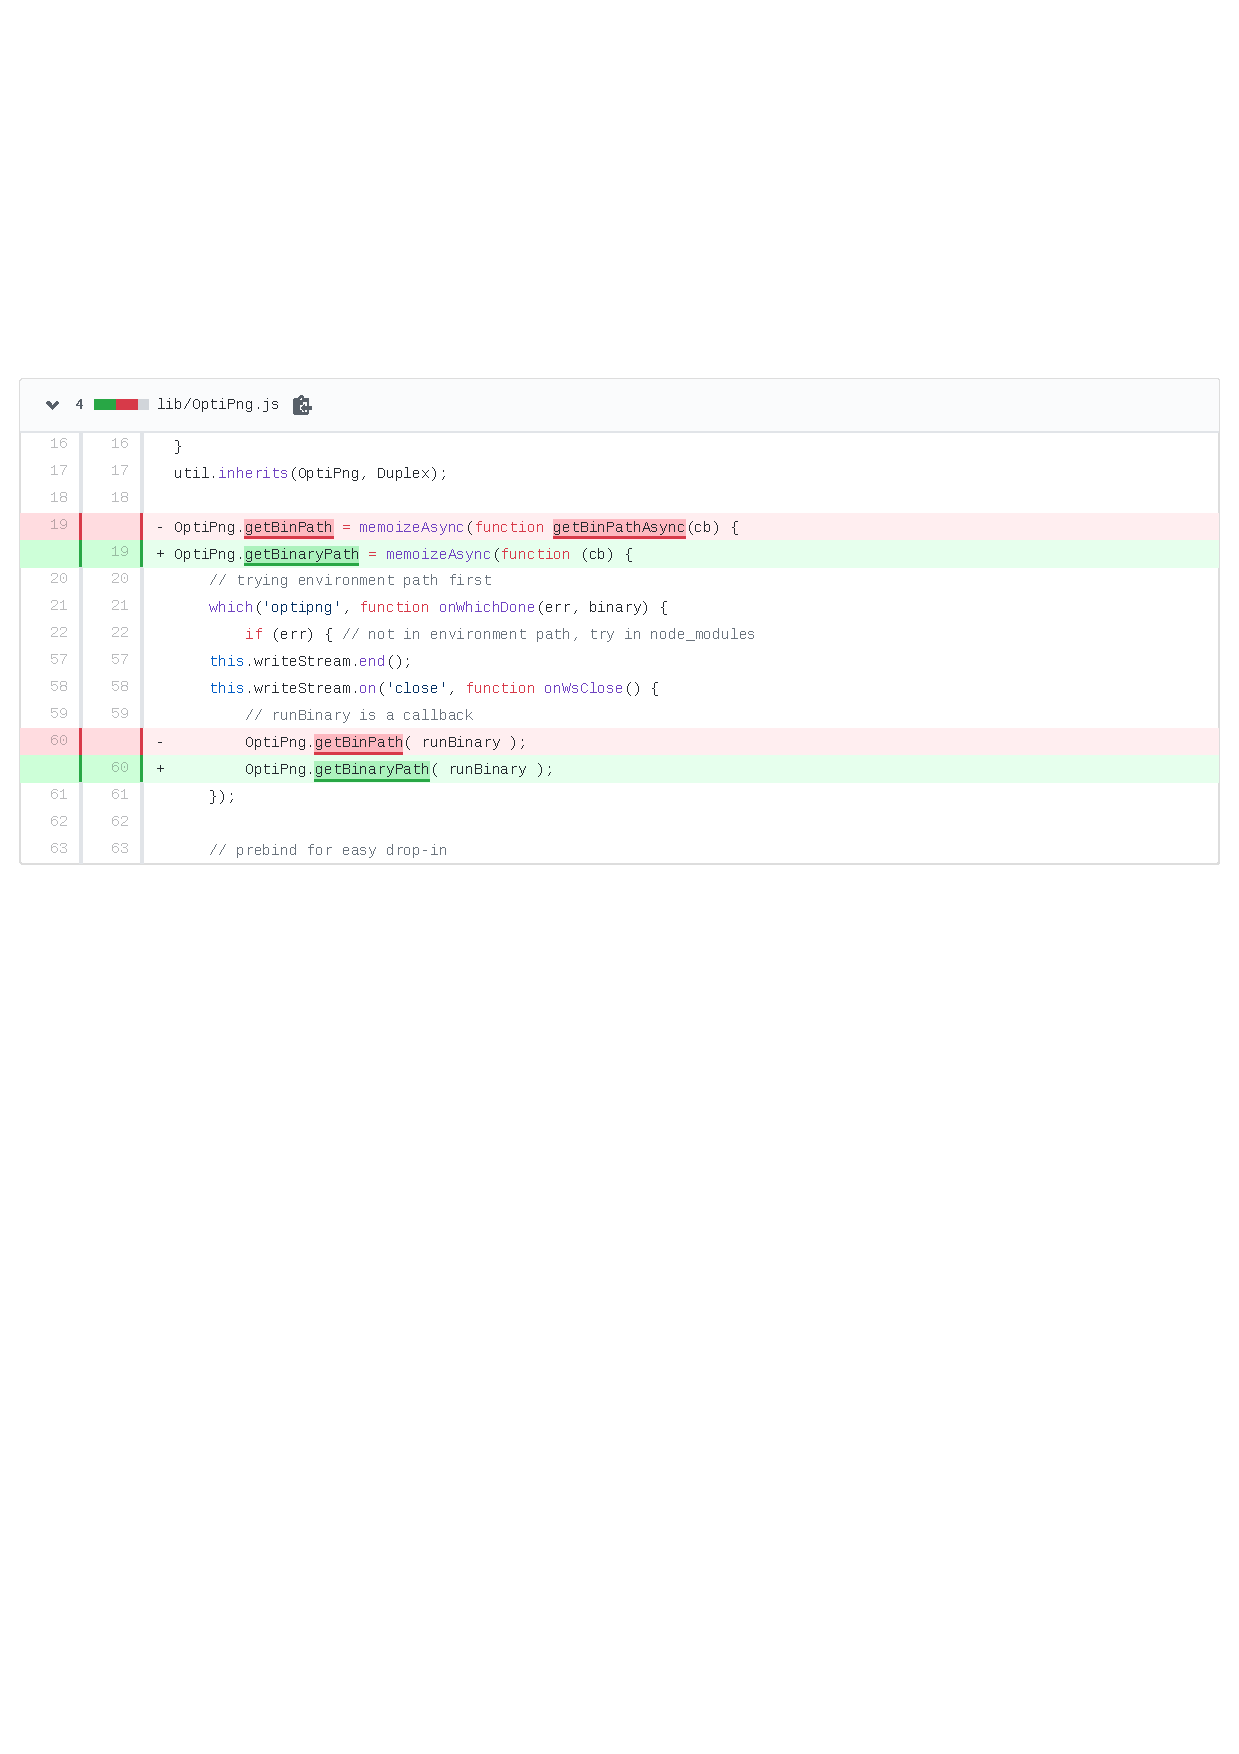
\includegraphics[scale=0.65]{figuras/bc_example.pdf}
    \caption{\textit{Commit} que corrigiu a \textit{breaking change}}
    \label{fig:bc_optipng}
\end{figure}{}

Alterações no código que causam \textit{breaking change} devem ser introduzidas em \textit{releases} versionadas com o incremento do nível \textit{major}, seguindo as especificações do Versionamento Semântico, definidos na Seção \ref{ref-teo:semver}. Assim, um cliente pode especificar se deseja ou não receber as \textit{releases} que contêm \textit{breaking change}. Entretanto, pesquisas relacionadas mostram que as \textit{breaking changes} são introduzidas erroneamente pelos provedores, assim, impactando os clientes. \citeonline{teorical_reference:bc_1} constatou que 9\% das \textit{releases} dos três pacotes com mais dependentes no \textit{npm} introduziram \textit{breaking changes} indevidamente e \citeonline{noregrets2018} apresentou uma ferramenta para detecção de \textit{breaking changes} e também constatou que 9\% das \textit{releases} introduziram \textit{breaking changes} quando não deveriam introduzir.
\daniel{Esses são os que eu coloquei nos trabalhos relacionados}

Além de quantificar as \textit{breaking changes} no ecossistema do \textit{npm}, este trabalho apresenta uma proposta para categorizar essas \textit{breaking changes} e verificar como os clientes se recuperam. Para isso, foi utilizado uma amostra representativa dos clientes no \textit{npm} e, para cada uma de suas \textit{releases}, foi verificado se houve alteração nas \textit{releases} que os clientes aceitavam dos provedores. Então, as versões dos provedores foram resolvidas para a última versão disponível até momento da publicação da \textit{release} do cliente e as \textit{releases} foram executadas através dos \textit{scripts npm install/npm test}. Após, foi feita uma análise manual no código das \textit{releases} que resultaram em erro para confirmar se o erro se tratava de uma \textit{breaking change} ou não. Por fim, foi feita uma análise nos repositórios dos provedores que introduziram as \textit{breaking change} para recuperar informações, tais como, tipo de \textit{breaking change}, tempo que levou até ser consertada, o nível da versão que a \textit{breaking change} foi introduzida/consertada.

Desse modo, o Capítulo \ref{cap:ref-teorico} contém a descrição de todos os termos utilizados ao longo desse trabalho. O Capítulo \ref{cap:qp} contém a motivação e o método para cada uma das questões de pesquisa. O Capítulo \ref{cap:metodologia} descreve sobre a manipulação dos dados que serão utilizados nessa pesquisa\daniel{serão ou foram?}. Por fim, o Capítulo \ref{cap:cronograma} apresenta o cronograma previsto das atividades faltantes para terminar esse trabalho.

% isso estava nos results
%\filipe{o erro sempre se manifesta no cliente, acho que o lance é que você consegue identificar se o erro foi proveniente de uma chamada a uma função do provedor ou do próprio cliente (ou algum outro provedor que não interessa à análise).}

%\filipe{breaking change (defeito no provedor) vs. manifestação da breaking change (manifestação do defeito do provedor no cliente)}
\chapter{Referencial Teórico}
\label{cap:ref-teorico}
Neste capítulo está descrito os fundamentos pertinentes a este trabalho. A Seção \ref{ref-teo:npm} apresenta o conceito e o funcionamento do \gls{npm} bem como a questão das dependências. A Seção \ref{ref-teo:prov_clie} distingue os termos \textit{provedor} e \textit{cliente}. Também para diferenciar termos, a Seção \ref{ref-teo:pac_rel_ver} discorre sobre \textit{pacote}, \textit{release} e \textit{versão}. A Seção \ref{ref-teo:semver} explica o que é \textit{Versionamento Semântico} e o \textit{SemVer} e como eles são utilizados no ecossistema do \gls{npm}. Porfim, a Seção \ref{ref-teo:breaking_change} conceitua e exemplifica as \textit{breaking changes}.

\section{\gls{npm}}
\label{ref-teo:npm}
O \gls{npm} é um gerenciador de pacotes para o \textit{Node.js}. Lançado em 2009, seu principal objetivo é facilitar o compartilhamento de códigos escritos em \textit{Javascript}. Atualmente, o \gls{npm} ocupa a posição de maior repositório para uma dada linguagem, com mais de 1 milhão de projetos\footnote{http://www.modulecounts.com/}. O \gls{npm} permite que, com apenas um simples comando, o usuário realize o download, publique, instale e desinstale pacotes diretamente de vários repositórios. A facilidade proporcionada pelo \gls{npm} corrobora para a grande popularidade do \textit{Javascript} e para que o compartilhamento de bibliotecas seja largamente utilizado, uma vez que 97\% dos aplicativos \textit{web} são oriundos do \textit{NPM}\footnote{https://blog.npmjs.org/post/180868064080/this-year-in-javascript-2018-in-review-and-npms}.

O ecossistema \gls{npm} estimula o compartilhamento de código entre aos pacotes. Por causa disso, dentre os demais repositórios, o \gls{npm} contém a maior distribuição de dependência entre os pacotes \cite{teorical_reference:npm_2}. Dessa maneira, como muitos pacotes estão dependendo mutuamente uns dos outros, há uma gigantesca rede de interconectividade entre os pacotes e, quando há um erro qualquer em algum desses pacotes, um grande número de outros pacotes podem ser afetados. Foi exatamente isso que ocorreu com um pacote chamado \textit{left-pad}\footnote{https://blog.npmjs.org/post/141577284765/kik-left-pad-and-npm}. Esse pacote foi removido do \textit{NPM} por seu desenvolvedor e impactou milhares de pacotes em apenas 2.5 horas, incluindo pacotes renomados como o \textit{babel}\footnote{https://github.com/babel/babel} e o \textit{atom}\footnote{https://github.com/atom/atom} que, devido ao grande número de dependentes, cascatearam o erro para inúmeros outros pacotes.
%In fact, 97\% of the code in a modern web application comes from npm

\section{Provedor e Cliente}
\label{ref-teo:prov_clie}
O pacote provedor é aquele que provê recursos ao pacote cliente, ou seja, contém interfaces públicas para acesso às suas funcionalidades. O termo \textit{pacote provedor} pode ser interpretado como \textit{bibliotecas} ou \textit{dependências}. Por exemplo, quando é executado o seguinte comando

\begin{lstlisting}[style=bash, label=cod:install:provider]
npm install mocha
\end{lstlisting}
o \gls{npm} salva o \textit{mocha} no \textit{package.json} como um provedor. Assim, o pacote \textit{mocha} é um provedor direto, pois foi instalado diretamente pelo usuário. Entretanto, as dependências do \textit{mocha} também são instaladas, mas de forma indireta pelo \gls{npm}. Estes outros pacotes são chamados de \textit{provedores indiretos}, pois não dependem que o usuário instale-os diretamente com o comando \textit{npm install}. A Figura \ref{fig:provider} mostra que, através do comando \textit{npm ls}, o pacote \textit{mocha} é um provedor direto do \textit{client}, pois o \textit{client} requer o \textit{mocha} para executar. Já o pacote \textit{glob} é um provedor direto do \textit{mocha}, e um provedor indireto do pacote \textit{client}.

\begin{figure}
    \centering
    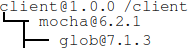
\includegraphics{figuras/provider_directly_undirectly.png}
    \caption{\textit{mocha} como provedor direto e \textit{glob} como indireto do \textit{client}}
    \label{fig:provider}
\end{figure}{}

Já o pacote cliente é aquele que está acessando as interfaces públicas do provedor. Quando uma \textit{break change} é introduzida pelo provedor -- direto ou indireto --, é sempre no pacote cliente que esta \textit{break change} se manifesta, causando o encerramento da execução. O pacote cliente é aquele que possui a responsabilidade de atualizar a versão de seus provedores no \textit{package.json} quando esses publicam uma \textit{release} com correções, enquanto que o pacote provedor possui a responsabilidade de indicar o nível de compatibilidade que sua nova \textit{release} está introduzindo \cite{teorical_reference:semver}.

\section{Pacote, \textit{Release} e Versão}
\label{ref-teo:pac_rel_ver}
Neste trabalho, a palavra \textit{pacote} refere-se a um \textit{software} hospedado no \gls{npm}. Esse \textit{software} contém seu nome, seus arquivos e suas versões. Por exemplo, quando nos referimos ao pacote \textit{mocha}, nos referimos à ideia genérica desse pacote, sem levar em consideração uma versão específica ou seu estado em algum instante, mas sim, apenas ao pacote como um todo.

Já a palavra \textit{release} designa o estado de um pacote em um determinado instante. Uma \textit{release} é denotada por uma versão específica desse pacote, isto é, um conjunto de arquivos distintos das demais \textit{releases}. Cada \textit{release} é acompanhada da publicação de uma nova versão do pacote no \gls{npm}.

Por fim, o termo \textit{versão} é utilizado para especificar e distinguir um determinado estado de uma \textit{release}. Uma \textit{versão} é uma \textit{string} no padrão \textit{SemVer} que identifica unicamente uma determinada \textit{release} e é utilizada pelo \gls{npm} no arquivo \textit{package.json} para especificar um \textit{range} de versões que o cliente aceita.

\section{Versionamento Semântico e \textit{SemVer}}
\label{ref-teo:semver}
O Versionamento Semântico\footnote{https://semver.org} é um padrão para versionamento de \textit{releases} de um projeto que considera o tipo de alteração introduzida na \textit{release}. As regras do Versionamento Semântico foram idealizadas por Tom Preston-Werner -- criador do \textit{GitHub} -- que incentiva todos os desenvolvedores à utilizarem este padrão, uma vez que as regras são baseadas em práticas comuns já utilizadas em projetos \cite{teorical_reference:semver}. Uma \textit{string} de versão no padrão do Versionamento Semântico possui os níveis \textit{<MAJOR>.<MINOR>.<PATCH>}\footnote{a \textit{string} pode ser estendida para versões \textit{beta, alpha, pre}, entre outros, tal como \textit{x.y.z-beta.0}}, que devem ser incrementados, quando o desenvolvedor publicar uma \textit{release}, de acordo com o seguinte critério:

\begin{itemize}
    \item \textit{MAJOR}: deve ser incrementado quando a \textit{release} introduz \textit{breaking changes};
    \item \textit{MINOR}: incrementado quando for adicionado melhorias/novas funcionalidades que mantenham a compatibilidade com as \textit{releases} anteriores; e
    \item \textit{PATCH}: deve ser incrementado quando a \textit{release} contém correção de \textit{bugs}.
\end{itemize}{}

Dessa maneira, se um projeto contém a sua última \textit{release} versionada como \textit{2.1.0}, por exemplo, o seu nível \textit{major} é o 2; o \textit{minor}, 1; e o \textit{patch}, 0. Ao publicar uma nova \textit{release}, se essa conter uma \textit{breaking change}, então deverá ser publicada com a versão \textit{3.0.0}; se for introduzida uma nova funcionalidade, \textit{2.2.0}; se houver uma correção de \textit{bugs}, \textit{2.1.1}.

O \textit{SemVer} é uma \textit{string} de versionamento que especifica um intervalo de versões, ou \textit{range}. Com o \textit{SemVer} é possível especificar quais são as \textit{releases} que o cliente aceita do seu provedor. Há vários padrões de \textit{range}\footnote{https://github.com/npm/node-semver\#ranges} especificados pelo \textit{SemVer}, mas os mais comuns, utilizados pelo \gls{npm}, são:

\begin{itemize}
    \item \textit{X-Ranges (*)}: este \textit{range} especifica para o \gls{npm} que o cliente aceita qualquer nova \textit{release} do provedor, até mesmo as \textit{releases} com \textit{breaking changes};
    \item \textit{Caret Ranges (\textasciicircum)}: este é o \textit{range} mais comum e o padrão do \gls{npm}. Com o \textit{Caret Range}, o cliente especifica que o \gls{npm} só deve descarregar novas \textit{releases} do provedor que contenham novas funcionalidades e correções de erros, mas que não contenham \textit{breaking changes}, ou seja, o cliente aceita todas as \textit{releases} das quais foram atualizadas os níveis \textit{patch} ou \textit{minor};
    \item \textit{Tilde Ranges (\textasciitilde)}: neste \textit{range}, o cliente especifica para o \textit{NPM} que somente as \textit{releases patch} do provedor são aceitas.
\end{itemize}{}

O \gls{npm} utiliza o padrão \textit{SemVer} no arquivo \textit{package.json} -- arquivo de configuração do projeto que contém todas os provedores e suas respectivas versões. Ao executar o comando \textit{npm install express --save}, para instalar o provedor \textit{express}\footnote{https://www.npmjs.com/package/express} por exemplo, o \gls{npm} -- além de descarregar este provedor -- irá salvar no \textit{package.json} o nome do provedor com sua versão atual em modo \textit{range}, de acordo com a Figura \ref{fig:dep_express}.

\begin{figure}
    \centering
    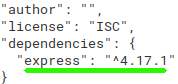
\includegraphics{figuras/dependencies_express.png}
    \caption{Modo como o \gls{npm} salva no \textit{package.json} a versão de uma dependência}
    \label{fig:dep_express}
\end{figure}{}

Com a informação do \textit{range} do provedor no \textit{package.json}, o cliente não precisa se preocupar com as novas atualizações de seus provedores, uma vez que o \gls{npm}, ao instalar novamente os provedores, sempre irá descarregar as \textit{releases} mais recentes que são aceitas pelo \textit{range SemVer}, especificado pelo cliente. Por padrão, o \gls{npm} especifica o \textit{Caret Range}, mas o cliente pode especificar outro \textit{range} manualmente no \textit{package.json} ou pode utilizar a opção \textit{--save-exact} para especificar a versão sem o \textit{range}, fazendo com que o \gls{npm} sempre instale esta versão específica.

\section{Breaking Change}
\label{ref-teo:breaking_change}
Uma \textit{break change} é uma alteração no pacote provedor que produz defeitos nos pacotes clientes \cite{teorical_reference:semver}. As \textit{break changes} surgem quando o pacote provedor, que previamente era executado com sucesso pelo cliente, publica uma \textit{release} que causa no cliente um comportamento inesperado, resultando em um erro. Durante o desenvolvimento de \textit{software}, os provedores precisam introduzir \textit{breaking changes}, pois quando só há \textit{releases} compatíveis com versões anteriores, o \textit{software} perde muitas oportunidades de evolução \cite{teorical_reference:bc_2}. Desta maneira, as \textit{break changes} são importantes para a evolução de um \textit{software}, uma vez que apenas \textit{releases} retro-compatíveis podem estagnar o \textit{software} limitando sua evolução. Assim, as \textit{breaking changes} também são sinônimos de evolução. Exemplo disso é o \textit{Node.js} que publica uma \textit{release} incrementando o nível \textit{major} a cada 6 meses\footnote{https://github.com/nodejs/node\#release-types}. Desta maneira, introduzir \textit{breaking changes} em níveis \textit{major} permite que os \textit{softwares} evoluam sem manter-se preso à versões anteriores.

Para evitar que os impactos de uma \textit{break change} afetem os clientes, os provedores publicam suas \textit{releases} com \textit{breaking changes} incrementando o nível \textit{major} da sua nova versão, seguindo a regra do Versionamento Semântico. Dessa maneira, os clientes de versões prévias que especificaram o provedor com o \textit{range caret} -- \textit{range} especificado por padrão pelo \gls{npm} -- ou o \textit{range tilde} não serão afetados por uma \textit{break change}. Porém, uma \textit{breaking change} pode ser introduzida em uma \textit{release} intencionalmente -- quando é atualizada o nível \textit{major} --, mas também pode ser introduzida inesperadamente -- quando é atualizado os níveis \textit{minor} ou \textit{patch}. Dessa maneira, o problema das \textit{breaking changes} está no fato do desenvolvedor introduzi-las em \textit{releases minor} ou \textit{patch}, resultando em defeitos nos clientes, uma vez que o cliente irá receber essa \textit{release} que contenha \textit{break changes} -- desde que o \textit{range} especificado para a versão do provedor aceite esta \textit{release} --, e se o cliente não espera ou não tratou previamente essa \textit{break change}, com certeza sua execução estará comprometida.

Um exemplo de \textit{breaking change} ocorreu na \textit{release optipng@0.2.0}: a \gls{API} \textit{OptiPng.getBinaryPath} foi renomada para \textit{OptiPng.getBinPath}\footnote{https://github.com/papandreou/node-optipng/pull/6}. Porém, a \gls{API} foi renomeada por engano e a \textit{release} errônea foi publicada em uma versão \textit{minor}, fazendo com que todos os clientes que tinham acesso àquela \gls{API} não a tivesse mais. Assim, o código \ref{cod:bc:optipng} executa normalmente com o \textit{optipng@0.1.1}, mas ao atualizar para o \textit{optipng@0.2.0}, este código sofre uma \textit{breaking change} -- o que não deveria acontecer com uma \textit{release minor}  -- conforme mostra a Figura \ref{fig:bc_optipng} (a).

\begin{lstlisting}[style=Javascript, label=cod:bc:optipng, caption={Código que sofre \textit{breaking change} do \textit{optipng}}]
var OptiPng = require('optipng');
var cb = {apply: () => {}};
OptiPng.getBinaryPath(cb);
\end{lstlisting}

Apesar de ser um erro facilmente detectável, esse foi consertado após 34 dias. E esta correção foi realizada em um \textit{commit}\footnote{https://github.com/papandreou/node-optipng/commit/a155f2b078224be18367847bbcbd3df3c379deea} no qual o desenvolvedor informou no comentário que a renomeação da \gls{API} ocorreu por engano, conforme a Figura \ref{fig:bc_optipng} (b), quando o desenvolvedor desfez a renomeação.

\begin{figure}
    \centering
    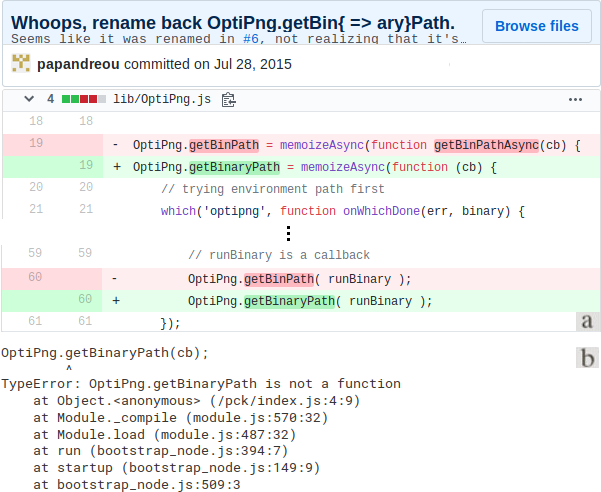
\includegraphics[scale=0.65]{figuras/bc_optipng.png}
    \caption{\textit{a}: \textit{stack trace} da \textit{break change}. \textit{b}: \textit{commit} que corrigiu a \textit{break change}}
    \label{fig:bc_optipng}
\end{figure}{}

\subsection{Casos de \textit{non-break changes}}
Além de alterações que resultam em \textit{breaking changes}, há algumas alterações que são causadas por provedores mas que, nessa pesquisa, não serão consideradas como \textit{breaking changes}. Essas alterações são:

\begin{itemize}
    \item Alterações da versão do \textit{Node.js}: o \textit{Node.js} atualizou o seu nível \textit{major} de \textit{0.x} para \textit{7.x} em apenas 3 anos\footnote{https://nodejs.org/en/download/releases}, mas isso não significa que os pacotes evoluíram seus códigos sempre para a última \textit{release} do \textit{Node.js}, e o inverso é valido, ou seja, os pacotes podem ter evoluído seus códigos na mesma frequência do \textit{Node.js}. Por exemplo, considere um pacote cliente executando no \textit{Node.js 0.x} com um provedor que evoluiu seu código para a sintaxe do \textit{Node.js 6.x}, que não é aceita no \textit{Node.js 0.x}. Desta maneira, não há uma versão do \textit{Node.js}  na qual seja possível executar o pacote cliente sem que no provedor seja manifestado um erro. Assim, erros nos provedores ocasionados por versões do \textit{Node.js} não serão considerados como \textit{break changes}, pois o erro foi causado pelo \textit{Node.js}, que não reconhece a sintaxe, e não pelo provedor;
    \item Exclusão de uma \textit{release}/\textit{provedor} do \gls{npm}: pelas regras do \gls{npm}, uma \textit{release} só pode ser removida até 72 horas após ter sido publicada\footnote{https://docs.npmjs.com/cli/unpublish\#description}. Entretanto, quando uma \textit{release} é removida do \gls{npm} e o cliente especificou aquela \textit{release}, isso gera um erro no \textit{script install}. Assim, o erro é causado pelo \gls{npm} que não consegue encontrar a \textit{release}, e não pelo provedor. No caso do provedor ter sido removido do \gls{npm} o caso é o mesmo: um provedor só pode ser removido após 72 horas. Entretanto, anterior ao acontecimento do \textit{left-pad}, os pacotes -- e \textit{releases} também -- podiam ser removidos do \gls{npm} em qualquer circunstância. Por isso, quando um pacote removido do \gls{npm} causar um erro, não será considerado como uma \textit{break change}.
    \item Alterações em serviços externos: os pacotes podem fazer uso de sistemas externos, tais como acesso à \textit{API}'s de sites e sistemas, e recuperar dados desses. Entretanto, ao longo do tempo, naturalmente, essas \textit{API}'s podem alterar seus dados, o que gera inconsistências em seus clientes. Mas esse tipo de erro não é considerado como uma \textit{break change}; e
    \item Cliente aceita \textit{releases} major do provedor: quando o cliente especifica em seu \textit{package.json} que aceita qualquer \textit{release} do provedor, através de um \textit{X-range}, o cliente então está aceitando \textit{releases} que foram introduzidas \textit{break changes}. Por isso, quando um cliente for impactado por uma \textit{break change} no provedor, e que foi corretamente introduzida em uma \textit{release major}, então o problema está no cliente que aceitou a \textit{break change} mas não a tratou.
\end{itemize}{}

\section{Trabalhos Relacionados}
\label{sec:related_works} % Esse capítulo e nome é apenas uma sugestão.
%% ATENÇÃO - veja com o seu orientador se você vai ter este capítulo e se este vai ter nome!
\chapter{Trabalhos Relacionados}
\label{cap:trabalhos:relacionados}

Apresente aqui os trabalhos similares ao seu trabalho ou que são importantes para o entendimento do seu trabalho...

(ATENÇÃO - veja com o seu orientador se você vai ter este capítulo e se este vai ter nome!)

\section{Uso de citações}
\label{cap:trabalhos:sec:relacionados:uso:citacoes}

Este é um exemplo do uso de citações no texto \cite{tomasulo:algorithm:5392028}.

Segundo \citeonline[p.~56]{Moore:2000:CMC:333067.333074} para citações textuais...

De acordo com o trabalho de \citeonline{Moore:2000:CMC:333067.333074} para citações textuais não tão específicas...


TEXTO TEXTO TEXTO TEXTO TEXTO TEXTO TEXTO TEXTO TEXTO TEXTO TEXTO TEXTO TEXTO TEXTO TEXTO TEXTO TEXTO TEXTO TEXTO TEXTO TEXTO TEXTO TEXTO TEXTO TEXTO TEXTO TEXTO TEXTO TEXTO TEXTO TEXTO TEXTO TEXTO TEXTO TEXTO TEXTO TEXTO TEXTO TEXTO TEXTO TEXTO TEXTO TEXTO TEXTO TEXTO TEXTO TEXTO TEXTO TEXTO TEXTO TEXTO TEXTO TEXTO TEXTO TEXTO TEXTO TEXTO TEXTO TEXTO TEXTO TEXTO TEXTO TEXTO TEXTO TEXTO TEXTO TEXTO TEXTO TEXTO TEXTO TEXTO TEXTO TEXTO TEXTO TEXTO TEXTO TEXTO TEXTO TEXTO TEXTO TEXTO TEXTO TEXTO TEXTO TEXTO TEXTO TEXTO TEXTO TEXTO TEXTO TEXTO TEXTO TEXTO TEXTO TEXTO TEXTO TEXTO TEXTO TEXTO TEXTO TEXTO TEXTO TEXTO TEXTO TEXTO TEXTO TEXTO TEXTO TEXTO TEXTO TEXTO TEXTO TEXTO TEXTO TEXTO TEXTO TEXTO TEXTO TEXTO TEXTO TEXTO TEXTO TEXTO TEXTO TEXTO TEXTO TEXTO TEXTO TEXTO TEXTO TEXTO TEXTO

%---------------------------------------------------%
\section{Considerações Finais}
\label{cap:trabalhos:relacionados:sec:consideracoes:finais}

Esta é uma sugestão de seção para dar um fechamento em cada uma dos capítulos.

(ATENÇÃO - veja com o seu orientador se é uma seção necessária (pois trate-se de estilo de escrita)) % Esse capítulo e nome é apenas uma sugestão.
%% ATENÇÃO - veja com o seu orientador se você vai ter este capítulo e se este vai ter nome!
\chapter{Proposta}
\label{cap:proposta}

Esse capítulo é mais indicado para TCC 1, no qual o aluno pode expor melhor qual é a proposta de seus trabalho para a realização do TCC 1 e 2. Bem como o cronograma para realização das atividades.

(ATENÇÃO - veja com o seu orientador se você vai ter este capítulo e se este vai ter nome!)

TEXTO TEXTO TEXTO TEXTO TEXTO TEXTO TEXTO TEXTO TEXTO TEXTO TEXTO TEXTO TEXTO TEXTO TEXTO TEXTO TEXTO TEXTO TEXTO TEXTO TEXTO TEXTO TEXTO TEXTO TEXTO TEXTO TEXTO TEXTO TEXTO TEXTO TEXTO TEXTO TEXTO TEXTO TEXTO TEXTO TEXTO TEXTO TEXTO TEXTO TEXTO TEXTO TEXTO TEXTO TEXTO TEXTO TEXTO TEXTO TEXTO TEXTO TEXTO TEXTO TEXTO TEXTO TEXTO TEXTO TEXTO TEXTO TEXTO TEXTO TEXTO TEXTO TEXTO TEXTO TEXTO TEXTO TEXTO TEXTO TEXTO TEXTO TEXTO TEXTO TEXTO TEXTO TEXTO TEXTO TEXTO TEXTO TEXTO TEXTO TEXTO TEXTO TEXTO TEXTO TEXTO TEXTO TEXTO TEXTO TEXTO TEXTO TEXTO TEXTO TEXTO TEXTO TEXTO TEXTO TEXTO TEXTO TEXTO TEXTO TEXTO TEXTO TEXTO TEXTO TEXTO TEXTO TEXTO TEXTO TEXTO TEXTO TEXTO TEXTO TEXTO TEXTO TEXTO TEXTO TEXTO TEXTO TEXTO TEXTO TEXTO TEXTO TEXTO TEXTO TEXTO TEXTO TEXTO TEXTO TEXTO TEXTO TEXTO TEXTO

%---------------------------------------------------%
\section{Cronograma de Atividades}
\label{cap:proposta:sec:cronograma}

(ATENÇÃO - Esta é apenas uma sugestão de elaboração de cronograma, veja com seu orientador!)

Em TCC 1 talvez seja interessante apresentar uma cronograma de realização das atividades da proposta que englobe as atividades do TCC 2.

Nesta seção são apresentadas as atividades a serem desenvolvidas para a execução da proposta. O cronograma de realização das tarefas é apresentado na Tabela~\ref{tab:cronograma}.

\begin{enumerate}
\item \textbf{Escrita do Projeto TCC 1.}
\item \textbf{Estudo de Técnicas...}
\item \textbf{Implementação da Ferramenta ...}
\item \textbf{Testes com o conjunto de \textit{benchmarks}.}
\item \textbf{Estudo de técnicas de Escalonamento de Tarefas.}
\item \textbf{Entrega do TCC 1}
\item \textbf{Apresentação do TCC 1}
\item \textbf{Realização de Experimentos.}
\item \textbf{Atividade do TCC 2}
\item \textbf{Escrita do TCC2}
\item \textbf{Entrega do TCC 2.}
\item \textbf{Apresentação do TCC 2.}
\end{enumerate}

\begin{table}[h!]
\renewcommand{\arraystretch}{1.3}
\caption{Cronograma de atividades}
\label{tab:cronograma}
\scalefont{0.9}
\begin{tabular}{|c|c|c|c|c|c|c|c|c|c|c|c|c|}
\hline
\multirow{2}{*}{\textbf{\textbf{Atividade}}} & \multicolumn{4}{c|}{\textbf{2014}}& \multicolumn{8}{c|}{\textbf{2015}} \\ \cline{2-13} 
& \multicolumn{1}{l|}{\textbf{Set}} & \multicolumn{1}{l|}{\textbf{Out}} & \multicolumn{1}{l|}{\textbf{Nov}} & \multicolumn{1}{l|}{\textbf{Dez}} & \multicolumn{1}{l|}{\textbf{Jan}} & \multicolumn{1}{l|}{\textbf{Fev}} & \multicolumn{1}{l|}{\textbf{Mar}} & \multicolumn{1}{l|}{\textbf{Abr}} & \multicolumn{1}{l|}{\textbf{Mai}} & \multicolumn{1}{l|}{\textbf{Jun}} & \multicolumn{1}{l|}{\textbf{Jul}} & \multicolumn{1}{l|}{\textbf{Ago}} \\ \hline
\textbf{1}  & X &   &   &   &   &   &   &   &   &   &   &  \\ \hline
\textbf{2}  & X & X & X & X &   &   &   &   &   &   &   &  \\ \hline
\textbf{3}  &   & X & X & X & X & X &   &   &   &   &   &  \\ \hline
\textbf{4}  &   &   & X & X & X & X &   & X & X &   &   &  \\ \hline
\textbf{5}  &   &   & X & X & X &   &   &   &   &   &   &  \\ \hline
\textbf{6}  &   &   & X & X & X & X & X & X & X & X &   &  \\ \hline
\textbf{7}  &   &   & X & X &   & X & X &   & X & X &   &  \\ \hline
\textbf{8}  &   &   &   & X & X &   & X & X &   & X & X &  \\ \hline
\textbf{9}  &   &   &   &   & X & X & X & X & X & X & X & X \\ \hline
\textbf{10} &   &   &   &   &   &   &   &   &   &   &   & X \\ \hline
\end{tabular}
\end{table}

%---------------------------------------------------%
\section{Considerações Finais}
\label{cap:proposta:consideracoes:finais}

Esta é uma sugestão de seção para dar um fechamento em cada uma dos capítulos.

(ATENÇÃO - veja com o seu orientador se é uma seção necessária (pois trate-se de estilo de escrita)) % Esse capítulo e nome é apenas uma sugestão (bom para TCC 1).
% ATENÇÃO - veja com o seu orientador se você vai ter este capítulo e se este vai ter nome!
\chapter{Metodologia}
\label{cap:metodologia}

\begin{itemize}
    \item RQ1: How often do breaking changes manifest in the client package?
\end{itemize}

A stack trace is a report that provides information about program subroutines. It is commonly used for certain kinds of debugging, where a stack trace can help software engineers figure out where a problem lies or how various subroutines work together during execution. When \textit{npm install} or \textit{npm test} results in an error, it raises a stack trace. All information about the error and the calls to providers are shown in the stack trace. Figure \ref{fig:trace} shows a generic example of a stack trace of one error.

\begin{figure}
    \centering
    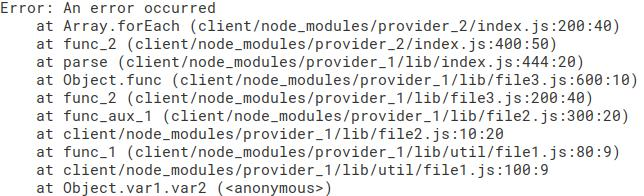
\includegraphics[scale=0.7]{figuras/stack_trace.jpeg}
    \caption{Generic stack-trace}
    \label{fig:trace}
\end{figure}{}

The stack trace is the base to analyze and an error.
All releases of any package that broke in the \textit{npm install} or \textit{npm test} were analyzed manually. The first step to analyze an error is differentiated between an error that wasn't caused by any provider, which is an error that occurred exclusively in the client package where the providers didn’t influence, and a breaking change error, that the errors occurred in provider package and it broke a client. There are two ways to conduct this step.

The first way is to take a look at the stack trace of the error and verify the calls to providers. When in the stack trace there isn't called to any providers, the error probably doesn’t refer a breaking change, because any provider was called in this error. So, the error is in the client code. To confirm this, the next commit in GitHub, after the release of the client, is verified. The objective is to verify if the error was fixed in any client commit. If true, the error is confirmed as a non-breaking change.
Some types of errors can be resolved in the code of the client. This error isn’t breaking change. Errors like \textit{SyntaxError} and \textit{ReferenceError}, where the client wrote the wrong code. Example:

\begin{lstlisting}[style=Javascript, label=cod:syntax:error, caption={Reference Error code in JavaScript}]
const a = 0 = 0;
\end{lstlisting}


In these errors, the npm raises a \textit{ReferenceError}. If the error is in the client code, nor is it necessary to look at \textit{GitHub}, because, for sure, the error is a non-breaking change. So, the code was fixed and the \textit{npm install} or \textit{npm test} is executed again to verify if any other error appeared.

The second way is when the errors can be a breaking change. This often occurs when the stack trace contains calls to any providers. However, providers like \textit{Mocha, Istanbul, Jasmine} and so on, that is, test frameworks, and task runners, like \textit{Grunt}, it is shown in stack trace but usually has no errors, because they only execute the files to test/tasks. So, when one of these providers is at the bottom of the stack tracer, they just called/execute the files/providers that contain the errors. Then, there’s a high probability that this error is a breaking change and this error can be caused by any provider.
To confirm this, the best place is in the \textit{GitHub}. The repository of the package contains all the information about the development. There are many ways to retrieve information. The easiest and most reliable way is to verify in a changelog file. These files, in general, are the \textit{CHANGELOG.md}, \textit{HISTORY.md} and others like this. These files contain the description of all changes about all packages releases. And many breaking changes are described there. For example, the release 5.0.0 of \textit{Mocha} contains a breaking change and was documented in \textit{CHANGELOG.md}. Figure \ref{fig:bc_documentation} show this documentation.

\begin{figure}
    \centering
    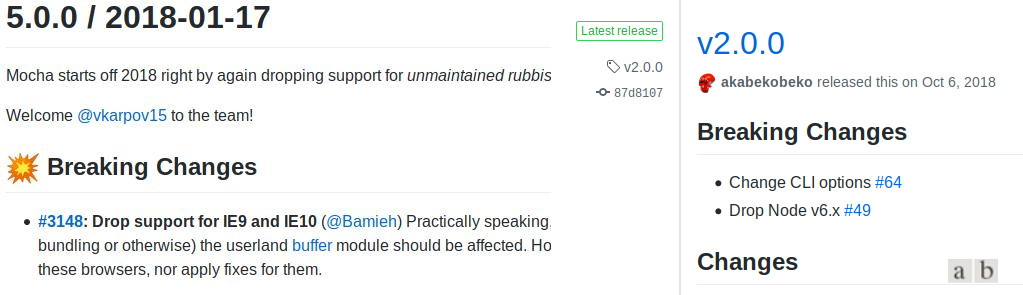
\includegraphics[scale=0.55]{figuras/bc_documentation.jpeg}
    \caption{Breaking Change documentation in README}
    \label{fig:bc_documentation}
\end{figure}{}

Other types of changelogs are the release notes. These are found in the comments of release. However, many and many repositories don’t contain a changelog file. Then, the next step is the search for any issue that contains some information about the error. In general, the issues contain much information, because of the developers and the owners of the package comment about the error. And more, many related issues are linked, increasing the number of information. Also, pull request works in the same way as issues.

Another important way is to install another release of the provider. So, it's possible to find out from which release the error started or which release the error was fixed. Also, there are other ways to verify if the error is in the provider. This is, compare the diff code between two provider releases; verify the provider commits; and change provider code.
The Figure \ref{fig:step_analyze} show a summary of these steps.

\begin{figure}
    \centering
    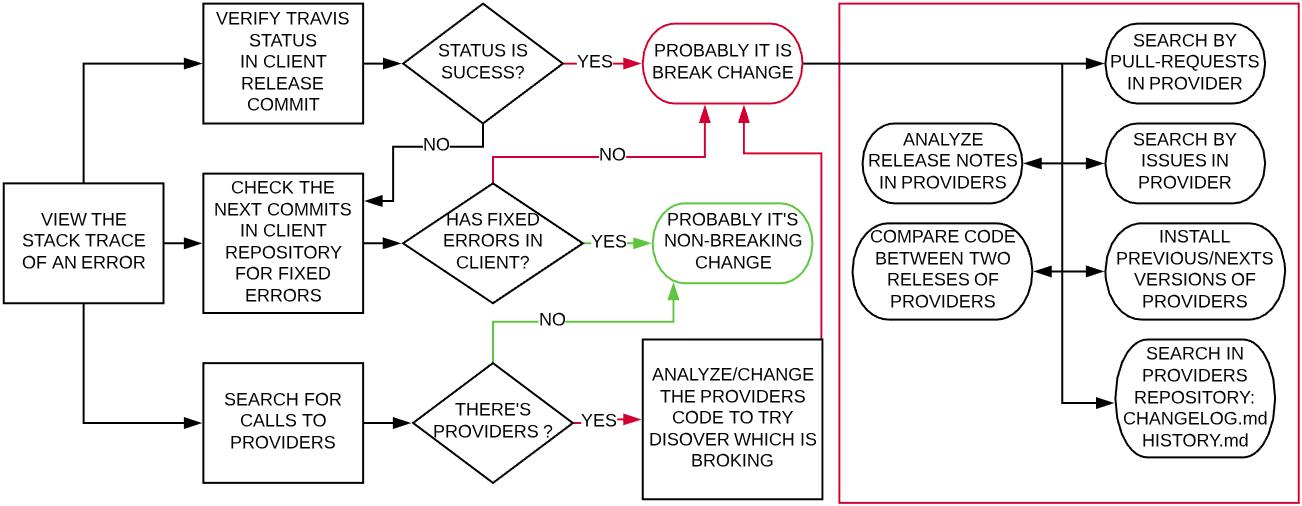
\includegraphics[scale=0.35]{figuras/step_analyze.jpeg}
    \caption{Steps to analyze an error}
    \label{fig:step_analyze}
\end{figure}
Some integrated systems can help to discover breaking changes. These systems are \textit{Travis, Jenkins, Codeship, CircleCI} and so on, and store the results of the npm install and npm test in the moment of a commit. It can help in the following way: if in the commit of a release the status of npm install or npm test was a success, and now is an error, then it occurred by a provider because the code of client is the same in the working tree and only the provider code was updated. However, just some of the sorted packages contain an integrated system.

Another detail is the packages that connect with some type of service likes, \textit{MySql, CouchDB, Redis} and so on. From all 385 packages, x required one of these services. When the \textit{npm install} or \textit{npm test} raises an error because of the connection, in manual analyze the required services were ability and re-executed the package. So, if the error was persister because the connection, the package was classified was \textit{Undiscovered Error}.

So, from all release analyze was saved many informations:

\begin{enumerate}
    \item Documentation about the error: issue, changelog, pull-request and so on;
    \item Who fixed the error: client or provider;
    \item How long did the error take to get fixed;
    \item Fixed in major, minor or patch; and
    \item In how many releases the error existed.
\end{enumerate}{}

Nor all information may be recovered. For example, if an error wasn't fixed, then neither the client nor the provider repaired the error.

\begin{itemize}
    \item RQ2: What issues in the provider package cause the manifestation of a breaking change?
\end{itemize}

For each error in \textit{npm install} or \textit{npm test}, it was manually analyzed. The objective is to do a grouping of similar errors and categorize then. For example, Figure \ref{fig:error_category} shows two errors in which one a function was renamed and the client tries to access the previous name.

\begin{figure}[!h]
    \centering
    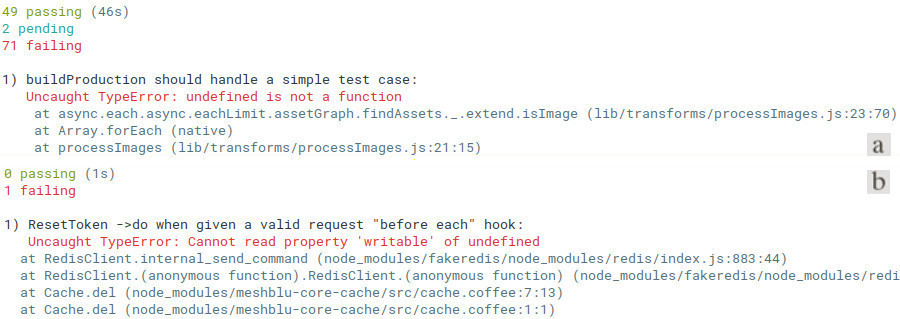
\includegraphics[scale=0.5]{figuras/error_category.jpeg}
    \caption{Two error caused by a renamed function}
    \label{fig:error_category}
\end{figure}

The first error in the Figure \ref{fig:error_category} is obvious: the client tries to access a variable like a function when it isn't a function. The second error talks about a property \textit{writable} that is access by an undefined object. There isn't any information about the function-related error, but, in manually analyze, it was observed that the provider change the name of a function. For this, in this code, the variable \textit{this.stream.writable} is undefined.

Once the provider causing the \textit{breaking change} has been discovered, there are several ways to find out the real reason that caused the error. These ways are described in Section \ref{cap:metodologia}. Then, all \textit{breaking changes} are classified based on his type.

\begin{itemize}
    \item RQ3: How do client packages recover from the manifestation of breaking change?
\end{itemize}

Since the customer recovers from the error, there are two ways to know how it recoverer. The first way is when the provider fixes his code and the client just updates the string of versioning in \textit{package.json}, if it needs. To the provider fixes the error, one issue may be done in his repository. The second way is when the client must do some work to fix the code. In this case, the client can fix the provider code and do a pull-request or change his code to work with the provider. And of course, may have cases that anyone does nothing. There is a breaking change and it’s never been fixed.

Where information about this RQ is retrieved is \textit{GitHub}. This information can be found at \textit{CHANGELOG, release-notes, issues,} and \textit{pull-requests}. If the \textit{changelog} contains information about fixed errors, in general, the related \textit{issues} are marked. From these \textit{issues}, a lot of more information can be recovered, like \textit{pull-requests} that are also marked in the \textit{issue}, other \textit{issues}, commentaries and more. All of this information can help us to discover which one -- client or provider -- fixed the \textit{breaking change} and how it was fixed.

\textit{Commits} are the alternative to \textit{issues} when the search is in the client repository. The \textit{commits} contain all changes in files and the all updates providers in \textit{package.json}. Commits message like \textit{update dependencies, fix dependencies, fix errors} an so on, suggests that something about any dependencies was fixed. This information is very important, because, since the provider was fixed and the client just updates it, the commit messages can tell the reason for this update - or downgrade.

%---------------------------------------------------%
\section{Considerações Finais}
\label{cap:metodologia:sec:consideracoes:finais}

Esta é uma sugestão de seção para dar um fechamento em cada uma dos capítulos.

(ATENÇÃO - veja com o seu orientador se é uma seção necessária (pois trate-se de estilo de escrita)) % Esse capítulo e nome é apenas uma sugestão.
%\chapter{Resultados}
\label{cap:results}

\section{RQ1. Com que frequência \textit{breaking changes} impactam nos pacotes clientes?}

Nesta Seção, encontram-se os resultados da análise manual voltados para responder a primeira questão de pesquisa. Nessa Seção estão os dados relacionados à quantificação das \textit{breaking changes}.

\subsubsection{\textbf{10.4\% dos clientes e 8.4\% das \textit{releases} sofreram \textit{breaking changes}}}

De todos os 384 clientes que tiveram seus testes executados, 40 (10.4\%) apresentaram algum caso de \textit{breaking changes}. Entretanto, os clientes podem ser impactados por mais de um tipo de erro, por exemplo, uma \textit{release} pode ser impactada por uma \textit{breaking change} e outra, por um erro interno. Assim, o mesmo cliente pode ser classificado em dois, ou mais, tipos de erros. Por isso, os resultados são melhores apresentados em função das \textit{releases}, uma vez que uma \textit{release} só pode ser impactada por apenas um tipo de erro. Desta maneira, analisando as \textit{releases}, de todas as \textit{2300} que tiveram seus testes executados, 902 (39.5\%) sofreram algum tipo de erro, que foram:

\begin{itemize}
    \item 433 (18.7\%) das \textit{releases} foram impactadas por erros internos;
    \item os casos particulares de \textit{breaking changes} impactaram 213 (9.2\%) das \textit{releases};
    \item as \textit{breaking changes} impactaram 193 (8.4\%) \textit{releases}; e
    \item 73 (3.2\%) das \textit{releases} foram impactadas por algum erro que não foi descoberto.
\end{itemize}{}

A Tabela \ref{tab:pre_res_rq1} contém os resultados em função das \textit{releases}.

\begin{table}[]
\centering
\begin{tabular}{lr}
\toprule
\textbf{Resultados}                & \textbf{\%} \\ \hline
Sucesso                                & 60.5\%      \\
Erros internos                         & 18.7\%      \\
Casos particulares de \textit{breaking changes} & 9.2\%       \\
\textit{Breaking changes}              & 8.4\%       \\
Não encontrados                        & 3.2\%       \\ \bottomrule
\end{tabular}\caption{Resultado da análise em cada caso de erro}
\label{tab:pre_res_rq1}
\end{table}

\subsubsection{Relação das \textit{releases} do cliente com os provedores e as \textit{breaking changes}}

Após analisar todos os casos de testes que resultaram em erro, foram constatados um total de 40 (10.4\%) clientes impactados por \textit{breaking changes}. Esses clientes sofreram com \textit{breaking changes} em pelo menos uma de suas \textit{releases}. Desde clientes com os testes executados em apenas uma \textit{release}, até os clientes com mais de 100 \textit{releases} foram impactados e, de maneira análoga, clientes com 1 provedor até clientes com mais de 100 provedores também foram impactados por \textit{breaking changes}. Observando apenas a amostra, é possível verificar que há uma correlação entre o número de \textit{releases} e o número de provedores, conforme a Figura \ref{fig:correlation_release_providers} apresenta. Nessa Figura, cada ponto representa um cliente com sua determinada quantidade de provedores e de \textit{releases}, respectivamente nos eixos \textit{x} e \textit{y}, também há uma regressão não-linear que caracteriza a correlação entre a quantidade de provedores e a quantidade de \textit{releases} que tiveram os testes executados, e por fim, há uma linha vertical e uma horizontal significando a mediana das \textit{releases} e dos provedores da amostra, respectivamente, sendo que essas medianas valem 3 e 9, assim, dividindo o plano cartesiano em 4 quadrantes. \daniel{havia alguns outliers que influenciavam um pouco no valor, mas usando um boxplot e um violin plot eu percebi que seria melhor usar a mediana à media. Mas a media daria 6 e 12}

Através da regressão não-linear percebe-se uma correlação entre o número de \textit{releases} e de provedores. Essa correlação caracteriza um crescimento no número de provedores a medida que o número de \textit{releases} aumenta, assim, quanto maior o número de \textit{releases}, maior o número de provedores que os clientes terão. Essa correlação também pode ser visualizada no quadrante em que estão os clientes que contêm seus provedores abaixo da mediana e suas \textit{releases} acima da mediana (inferior direito). Esse é o quadrante com a menor concentração de clientes, contendo apenas 7\%, e, visivelmente, percebe-se que, conforme as \textit{releases} aumentam, o número de provedores aumenta, tanto que o maior cliente contém 40 \textit{releases}, e os clientes que contém mais de 40 \textit{releases} possuem uma quantidade de provedores acima da mediana.

\begin{figure}
    \centering
    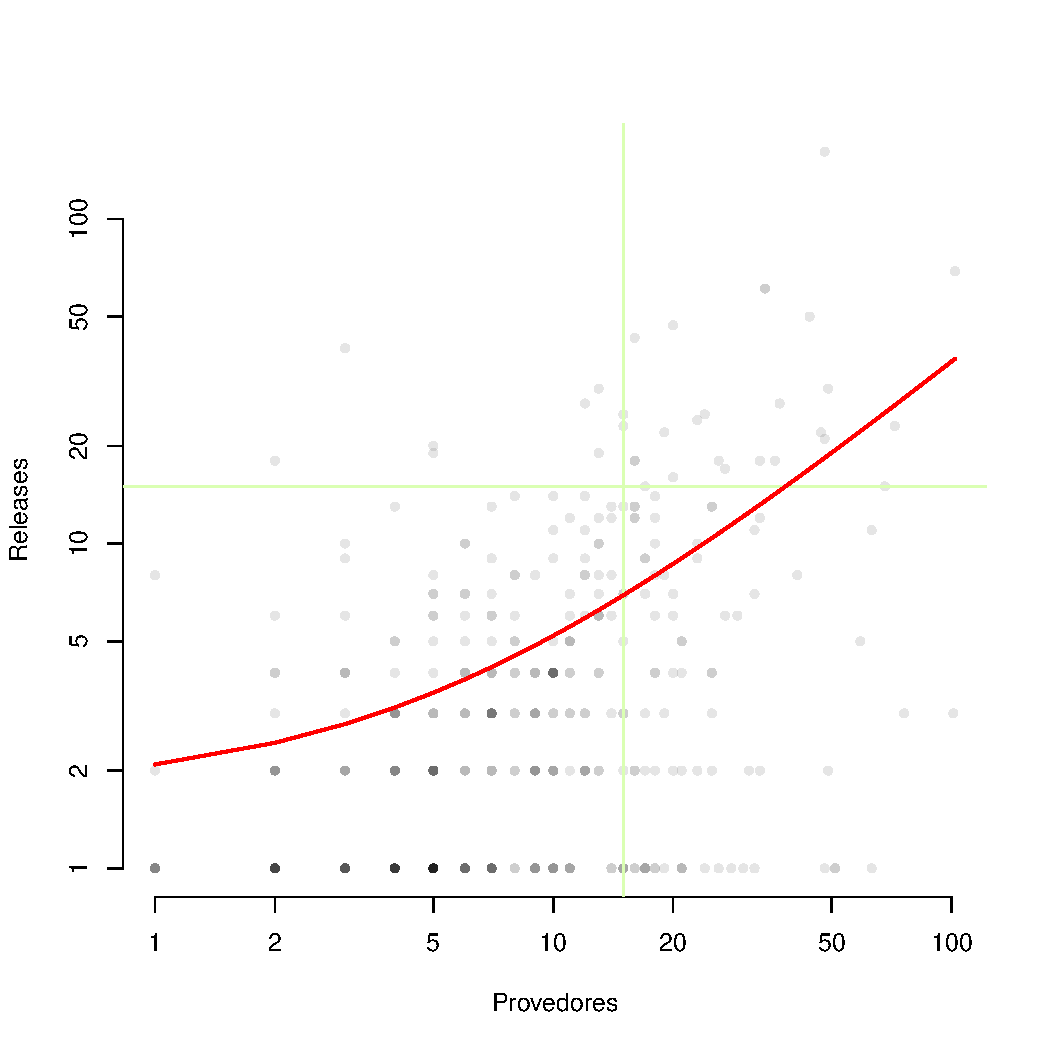
\includegraphics[scale=0.6]{figuras/correlation_release_providers.pdf}
    \caption{Correlação entre a quantidade de \textit{releases} e de provedores da amostra}
    \label{fig:correlation_release_providers}
\end{figure}{}

A análise dos clientes com \textit{breaking changes} se encontra na Figura \ref{fig:result_rq1_releases_affecteds}, que correlaciona a quantidade de provedores com a quantidade de \textit{releases} que foram executados os testes, respectivamente no eixo \textit{y} e \textit{x}. Nessa Figura, assim como na Figura anterior, estão dispersos os clientes da amostra e, em destaque, os que sofreram com \textit{breaking changes}. O tamanho dos círculos  representam a proporção de \textit{releases} dos clientes que foram impactadas, ou seja, a quantidade de \textit{releases} com os testes executados pela quantidade de \textit{releases} impactadas por \textit{breaking changes}. Assim, quanto maior os círculos vermelhos, maior o impacto das \textit{breaking changes}. Por fim, há uma regressão não-linear da relação dos provedores com as \textit{releases} dos clientes afetados com \textit{breaking changes} e uma linha vertical e uma horizontal significando a mediana das \textit{releases} e dos provedores que foram impactados por \textit{breaking changes}, respectivamente, e essas medianas valem 8 e 14, assim, dividindo o plano cartesiano em 4 quadrantes. A Figura \ref{fig:percentage_clients_bc} contém a porcentagem de clientes de cada quadrante da Figura \ref{fig:result_rq1_releases_affecteds}. Por exemplo, o quadrante superior esquerdo da Figura \ref{fig:result_rq1_releases_affecteds} contém 17.2\% dos clientes da amostra, como pode ser visto no seu respectivo eixo (\textit{Sup. esquerdo}) na Figura \ref{fig:percentage_clients_bc}, e desses 17.2\%, 10.6\% foram afetados com \textit{breaking changes}, ou seja, esses 10.6\% são a porcentagem de clientes impactados por \textit{breaking changes} nesse determinado quadrante.

\begin {figure} [h!]
   \centering
   \mbox {
        \subfigure[]{\label{fig:result_rq1_releases_affecteds} 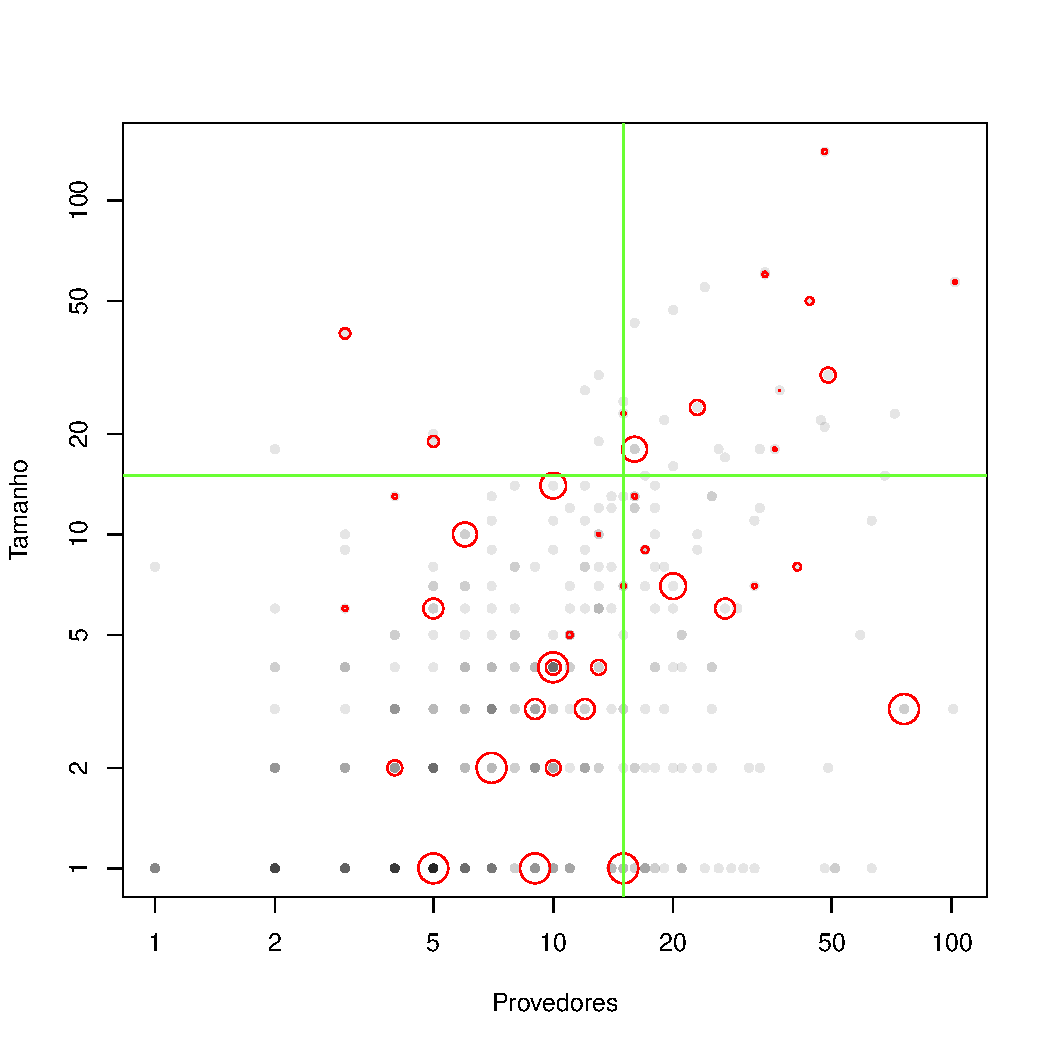
\includegraphics[scale=0.45]{figuras/result_rq1_releases_affecteds.pdf}}\quad
        \subfigure[]{\label{fig:percentage_clients_bc} 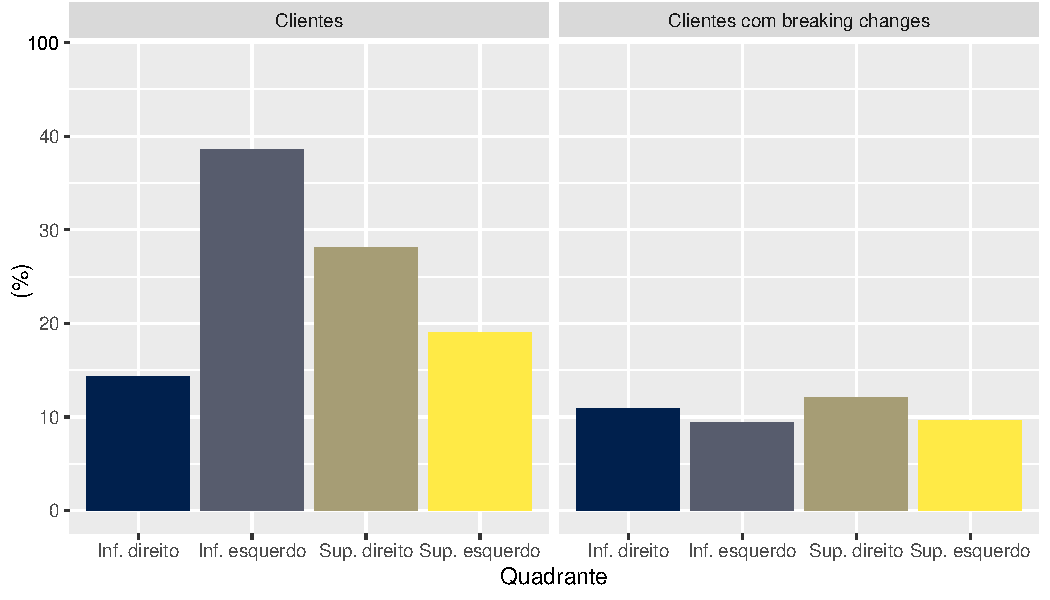
\includegraphics[scale=0.3]{figuras/percentage_clients_bc.pdf}}
    }
    \caption{(a) Dispersão das \textit{break changes} em função da quantidade de \textit{releases} e de provedores; (b) percentual de clientes de cada quadrante da Figura \ref{fig:result_rq1_releases_affecteds}}
    \label{fig:result_rq1_once_twice_three}
\end{figure}

Através da regressão não-linear da Figura \ref{fig:result_rq1_releases_affecteds}, verifica-se que a manifestação das \textit{breaking changes} está relacionada com o número de \textit{releases} executadas e com o número de provedores, uma vez que a regressão é crescente conforme a quantidade de provedores e de \textit{releases} aumentam. Mas, no quadrante em que há a maior concentração de clientes (inferior esquerdo), com 64.6\% dos clientes da amostra, há a mais baixa porcentagem de casos de \textit{breaking changes}, com um total de 5.6\% de ocorrências, mesmo sendo o quadrante com mais clientes. Neste caso, conclui-se que a manifestação de \textit{breaking changes} para clientes com um quantidade abaixo da mediana de provedores e de \textit{releases} não é comum, ou seja, os clientes com poucos provedores e poucas \textit{releases} foram os menos impactados. Ainda analisando a Figura \ref{fig:percentage_clients_bc}, é possível verificar que a manifestação de \textit{breaking changes} está fortemente relacionada com a quantidade de \textit{releases} do cliente. Essa relação está no fato de que os quadrantes com os maiores percentuais de ocorrência de \textit{breaking changes} são os quadrantes \textit{superior direito} e \textit{inferior direito}, com 30.2\% e 22.2\% de seus clientes impactados, respectivamente, e a Figura \ref{fig:result_rq1_releases_affecteds} mostra que esses dois quadrantes são os que possuem os clientes com a quantidade de \textit{releases} acima da mediana. E, como a quantidade de \textit{releases} que tiveram seus testes executados está diretamente relacionada com as atualizações dos provedores -- os testes das \textit{releases} só foram executados quando havia algum provedor que tinha publicado uma nova \textit{release} --, conclui-se que a manifestação das \textit{breaking changes} é motivada pela frequência com que os provedores publicam suas \textit{releases}. Clientes que possuem grande quantidade de provedores, mas que possuem poucas \textit{releases} com seus testes executados, não são tão impactados por \textit{breaking changes} quanto os clientes que tiveram uma grande quantidade de \textit{releases} com testes executados.

\subsubsection{Fase de desenvolvimento para a introdução das \textit{breaking changes}}

Um provedor evolui conforme os seus desenvolvedores publicam \textit{releases}, sejam essas contendo correções, melhorias ou novas funcionalidades. Durante o desenvolvimento dos provedores, os desenvolvedores tendem a ter uma visão mais clara de como evoluir seus provedores evitando \textit{breaking changes}, assim as \textit{releases} tendem a ser menos instáveis. Contudo, até mesmo provedores estáveis e com código bem desenvolvido podem introduzir \textit{breaking changes} após muito tempo de desenvolvimento, mas em um estágio avançado de desenvolvimento os provedores deveriam ser mais estáveis. Entretanto, nem sempre isso acontece. A Figura \ref{fig:providers_releases_bc} apresenta a porcentagem de cada provedor que foi desenvolvida até o surgimento da \textit{breaking change}, ou seja, em qual estágio de desenvolvimento a determinada \textit{breaking change} foi introduzida. Dessa análise foram removidos quatro provedores que introduziram \textit{breaking changes} na primeira \textit{release} e dois que introduziram \textit{breaking changes} além da data da coleta de dados, descrita na Seção \ref{sec:col_base}. Assim, foram analisados 30 provedores. \daniel{Eu não considerei os casos introduzidos na primeira release porque o provedor praticamente não foi desenvolvido ainda. Será que devo considerar esses 4 casos?}

\begin{figure}
	\centering
	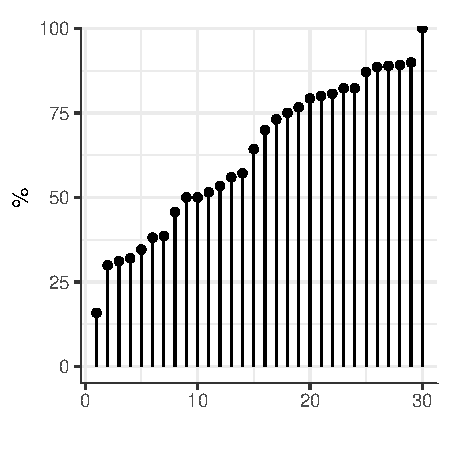
\includegraphics{figuras/providers_releases_bc.pdf}
	\caption{Fase de desenvolvimento do provedor no qual a \textit{breaking change} foi inserida}
	\label{fig:providers_releases_bc}
\end{figure}{}

Através da Figura \ref{fig:providers_releases_bc} percebe-se que as \textit{breaking changes} são mais introduzidas em um estágio avançado do provedor, uma vez que apenas 8 (26.7\%) provedores introduziram \textit{breaking changes} antes do desenvolvimento chegar a 50\%.  Isso significa que esses provedores introduziram as \textit{breaking changes} em suas primeiras \textit{releases}, e isso pode ser muito desfavorável para os provedores e pode acarretar na perca de clientes, uma vez que se os provedores possuem poucas \textit{releases}, os clientes podem não ter a opção de realizar um \textit{dowgraded} para uma \textit{release} estável dos provedores e aguardar a publicação de uma \textit{release} com a correção da \textit{breaking change} pode não ser viável e isso pode induzir o cliente a trocar de provedor.

Os provedores que introduziram \textit{breaking changes} entre os 50\% e antes dos 75\% de desenvolvimento foram 9 (30\%). Nessa fase de desenvolvimento, os provedores deveriam ser bem estáveis e não apresentar \textit{breaking changes}, uma vez que o desenvolvimento está mais avançado e os clientes podem estar usando várias interfaces dos provedores, e ter que alterar seu provedor quando se utiliza muitos recursos dele é algo muito custoso para o cliente. Entretanto, como mais da metade das \textit{releases} dos provedores já foram publicadas, o cliente pode optar em realizar um \textit{dowgraded} para uma versão estável dos provedores enquanto a correção da \textit{breaking change} não é publicada. Assim, as \textit{breaking changes} nessa fase de desenvolvimento são mais fáceis de tratar por parte do cliente.

Por fim, os provedores que introduziram \textit{breaking changes} após os 75\% de desenvolvimento foram 13 (43.3\%) provedores. Nessa fase de desenvolvimento o cliente pode facilmente realizar um \textit{dowgraded} para uma \textit{release} estável e, por ser introduzida em uma fase mais recente de desenvolvimento, o provedor pode ter alcançado vários clientes e ser motivado a consertar a \textit{breaking change} com mais rapidez.
\section{RQ2. Como os pacotes provedores introduzem \textit{breaking changes} em uma \textit{release}?}
\label{sec:qp2:results}

\subsubsection{Categorias de \textit{Breaking changes}}
Ao todo, foram 45 casos de \textit{breaking changes} distribuídas em 40 clientes. Todos esses casos foram agrupados em 8 diferentes categorias das quais se encaixavam os casos semelhantes. A Tabela \ref{tab:bc_category} apresenta cada uma dessas categorias, bem como a quantidade de pacotes e a quantidade de \textit{releases} que cada categoria atingiu.

\begin{table*}\centering
	\begin{tabular}{lrrrrr} \toprule
		\textbf{Categoria} & \multicolumn{2}{c}{Pacotes} & \phantom{ab} & \multicolumn{2}{c}{\textit{Releases}}
		\\
		\cmidrule{2-3} \cmidrule{5-6}
		& afetados & (\%) && afetadas & (\%) \\ \midrule
		Alteração de regras          & 14              & 31,11 && 67                          & 34,71 \\
		Provedores incompatíveis     & 11              & 24,44 && 37                          & 19,17 \\
		Alteração de tipo de objeto  & 7               & 15,55 && 22                          & 11,39 \\
		Objeto indefinido            & 4               & 8,88  && 25                          & 12,95 \\
		Código não-atualizado        & 3               & 6,66  && 25                          & 12,95 \\
		Código errado                & 3               & 6,66  && 11                          & 5,69  \\
		Renomeação de função         & 2               & 4,44  && 2                           & 1,03  \\
		Arquivo não encontrado       & 1               & 2,22  && 4                           & 2,07  \\ \hline
		\textbf{Total}               & \textbf{45}     &       && \textbf{193}              &       \\
		\bottomrule
	\end{tabular}
    \caption{Categorias dos casos de \textit{breaking changes}}
    \label{tab:bc_category}
\end{table*}

A seguir, encontra-se uma descrição sobre cada categoria e um exemplo de como os pacotes dessa determinada categoria foram afetados.

\begin{itemize}
    \item \textbf{Alteração de regras}: este caso foi o principal que impactou os pacotes. Essa categoria contém os casos de \textit{break change} no qual os provedores possuíam um determinado comportamento, mas alteraram algumas de suas regras/funcionalidades e impactaram os seus clientes. Não foi uma simples alteração no código, tal como uma alteração de tipo de variáveis, ou um código escrito de maneira errada, mas sim uma regra no qual o cliente tinha como sólida, foi alterada. Por exemplo, o pacote \textit{request@2.17.0} -- essa \textit{release} não existe mais no \textit{npm}, mas a alteração se manteve -- introduziu uma alteração em seu código\footnote{https://github.com/request/request/commit/d05b6ba72702c2411b4627d4d89190a5f2aba562\#diff-168726dbe96b3ce427e7fedce31bb0bcR857}, como pode ser visto na Figura \ref{fig:bc_category_change_rule_1}.

    \begin{figure}
        \centering
        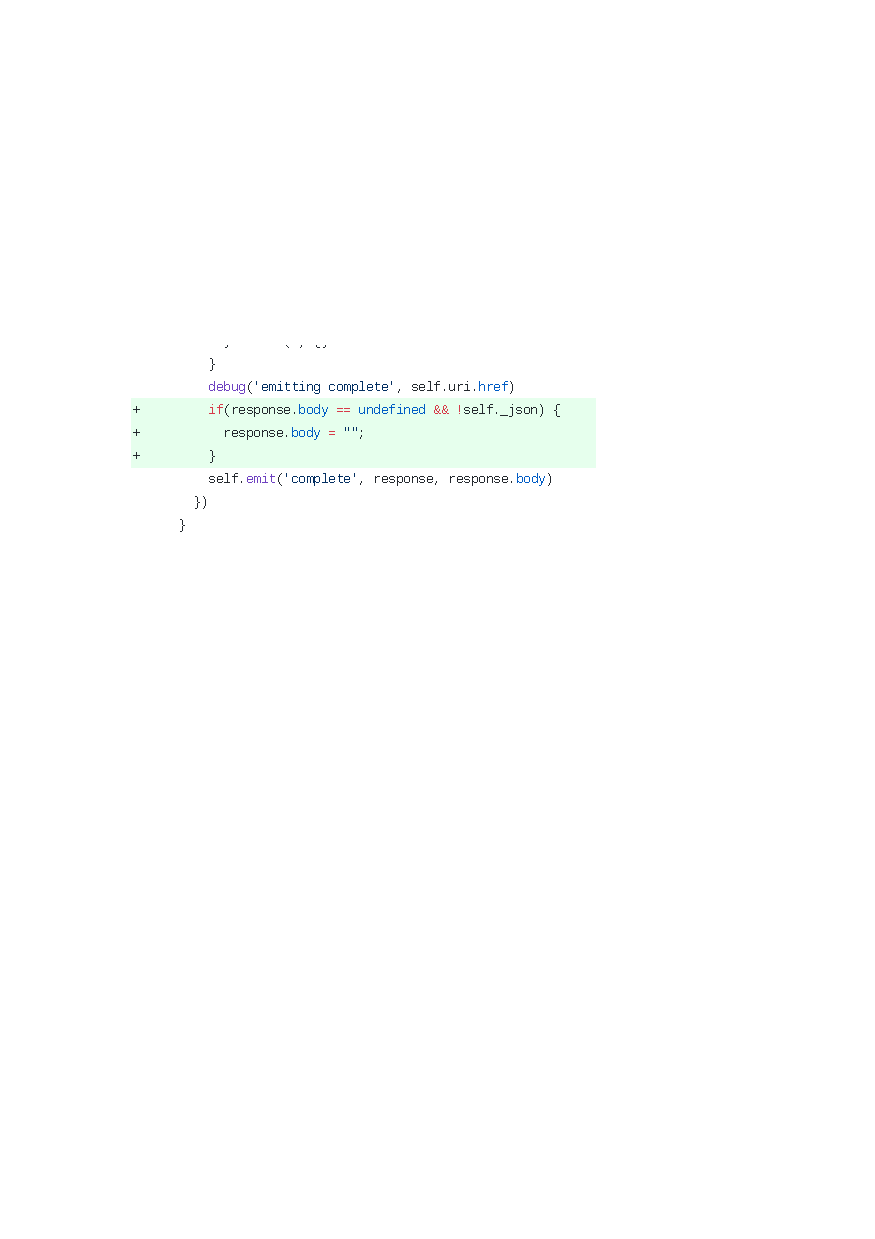
\includegraphics{figuras/bc_category_change_rule_1.pdf}
        \caption{Alteração de regra de funcionamento do \textit{request}}
        \label{fig:bc_category_change_rule_1}
    \end{figure}{}

    Nesse caso, o \textit{request} adiciona uma \textit{string} vazia ao invés de manter \textit{undefined} o corpo de uma requisição. Esse caso do \textit{request} ocorreu exatamente como foi explicado por \citeonline{Foo:2018:ESC:3236024.3275535} dizendo que os pacotes evoluem independentemente dos clientes. Essa alteração na regra do \textit{request} reflete em uma evolução do pacote, mas o cliente não esperava essa alteração e confiava que o corpo da resposta fosse retornado como \textit{undefined} em caso de erro, por isso o cliente resultou em um erro.

    \item \textbf{Provedores incompatíveis}: nessa categoria, há um provedor direto A e um provedor indireto B envolvido, o qual alterou o seu código, o que não gerou um erro, mas provocou no provedor A um comportamento inesperado, ou seja, o provedor B passou a ser incompatível com o provedor A. Nessa categoria, nenhum dos provedores contém um erro, mas sim uma incompatibilidade. Um exemplo disso ocorreu com os pacotes \textit{babel-eslint}\footnote{https://www.npmjs.com/package/babel-eslint} e \textit{escope}\footnote{https://www.npmjs.com/package/escope}, sendo o pacote \textit{escope} é um provedor indireto do \textit{babel-eslint}.

    \begin{figure}
        \centering
       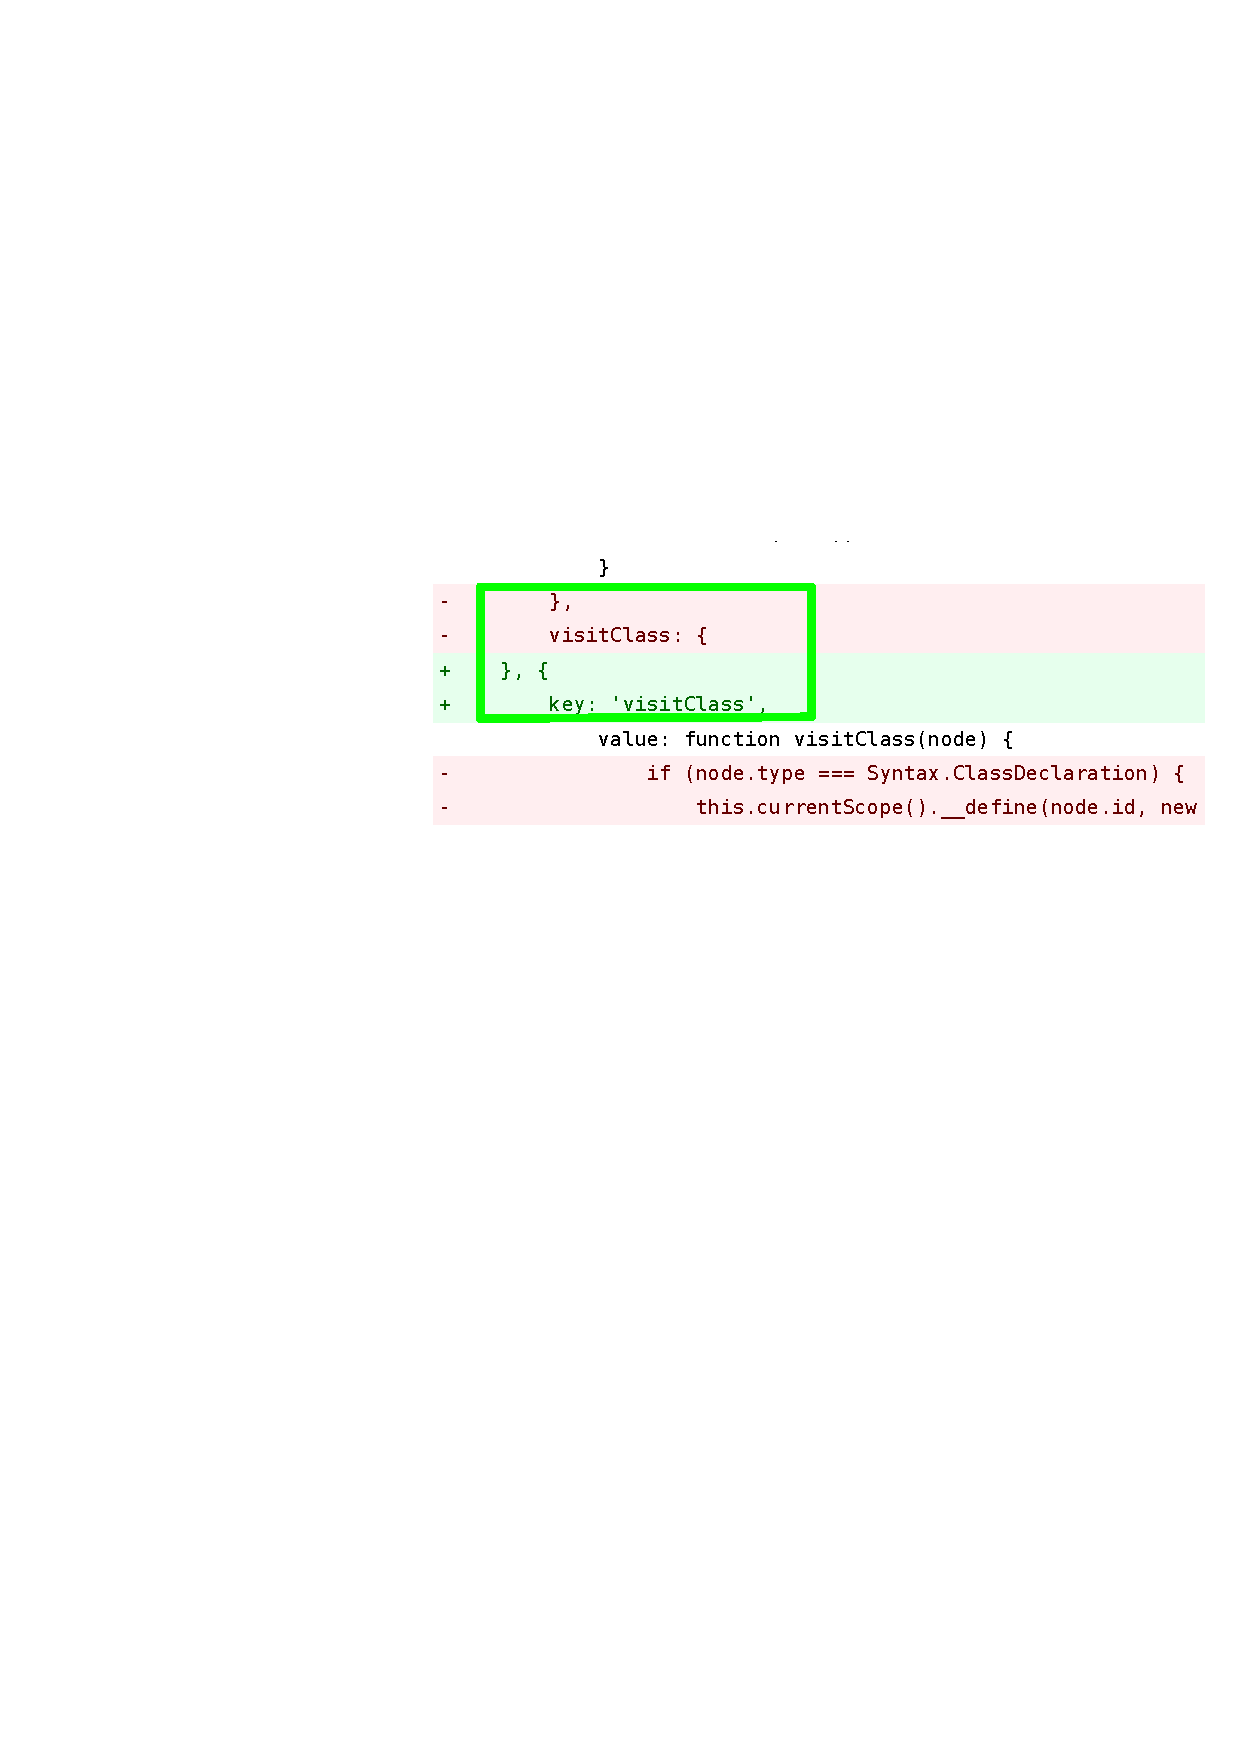
\includegraphics[scale=0.7]{figuras/bc_category_incompatibles_providers.pdf}
        \caption{Alteração de código do \textit{escope}}
        \label{fig:bc_category_incompatibles_providers}
    \end{figure}{}

    A \textit{release escope@3.4} realizou uma alteração no seu código, de acordo com a Figura \ref{fig:bc_category_incompatibles_providers}, mas que não reflete em um erro. Essa alteração impactou diretamente o pacote \textit{babel-eslint}, mesmo o pacote \textit{escope} não sendo um provedor direto do \textit{babel-eslint} e não ter introduzido um erro\footnote{https://github.com/estools/escope/issues/99\#issuecomment-178151491}. Com isso, há uma incompatibilidade entre os provedores e essa incompatibilidade precisou ser corrigida pelo \textit{babel-eslint} e não pelo \textit{escope}. Essa foi a \textit{breaking change} que mais surgiu na análise manual pois, dos 45 casos, 6 (13.3\%) refletiam essa incompatibilidade, uma vez que o \textit{babel-eslint} é provedor direto de 5.8\% de todo o conjunto de dados.

    \item \textbf{Alteração de tipo de objeto}: essa é uma categoria de \textit{break changes} facilmente detectável em linguagens fortemente tipadas, mas no \textit{Javascript} representam um tipo de \textit{break change} que, por muitas vezes, pode nem afetar o código do cliente. Mas, neste trabalho, foram detectados 7 (15.5\%) de casos nos quais os provedores alteraram o tipo de alguma variável.

    \begin{figure}
        \centering
        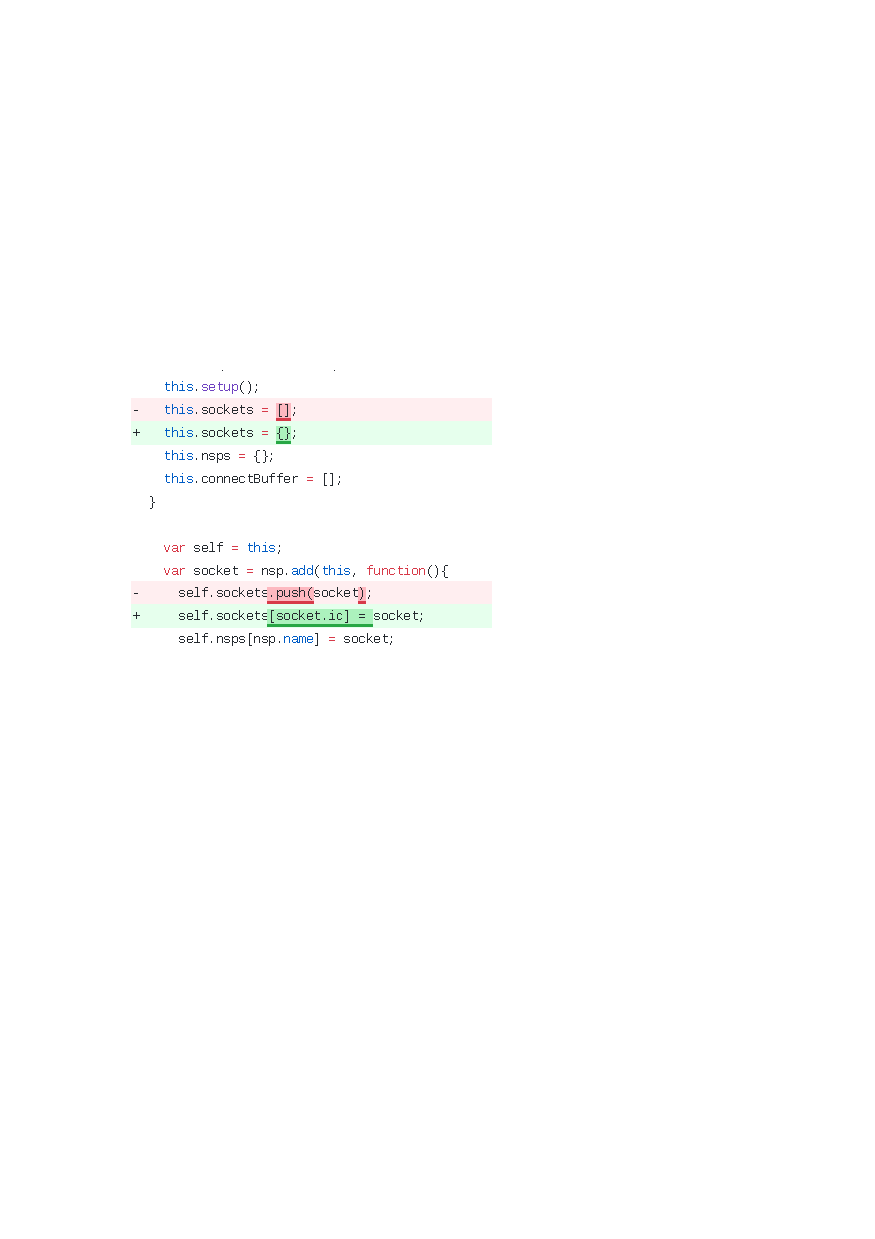
\includegraphics[scale=0.9]{figuras/bc_category_change_type.pdf}
        \caption{Alteração de um tipo \textit{array} para \textit{object}}
        \label{fig:bc_category_change_type}
    \end{figure}{}

    Na Figura \ref{fig:bc_category_change_type} o provedor \textit{socket.io}\footnote{https://www.npmjs.com/package/socket.io} alterou alguns \textit{arrays} para \textit{object}\footnote{https://github.com/socketio/socket.io/commit/b73d9bea4efb48277eee685763026ff2df5a79ab}. Anteriormente, os clientes iteravam nesses \textit{arrays}, mas após essa alteração, os clientes foram afetados.

    \item \textbf{Objeto indefinido}: por vezes, os códigos podem estar todos corretos, mas então o provedor tenta acessar uma variável que não existe. Esta categoria de \textit{break change} representa os casos no qual os provedores tentaram obter acesso à alguma variável/objeto, mas que não existiam. Esses erros são os que facilmente podem ser consertados/evitados apenas adicionando o código da Listagem \ref{cod:undefined_object}:

    \begin{lstlisting}[style=bash, label=cod:undefined_object]
    this.var = this.var || {};
    \end{lstlisting}

    Esse tipo de erro surgiu no pacote \textit{ember-cli-htmlbars-inline-precompile}\footnote{https://www.npmjs.com/package/ember-cli-htmlbars-inline-precompile}, no qual o desenvolvedor tenta acessar uma variável que não estava disponível. Mas, assim como o desenvolvedor já havia feito com as demais variáveis da Figura \ref{fig:bc_category_undefined_object}, uma simples alteração no código foi o suficiente\footnote{https://github.com/ember-cli/ember-cli-htmlbars-inline-precompile/pull/5/commits/b3faf959fcea8e5b928f4fa28bf6572534968d81\#diff-168726dbe96b3ce427e7fedce31bb0bcR13}.

    \begin{figure}
        \centering
        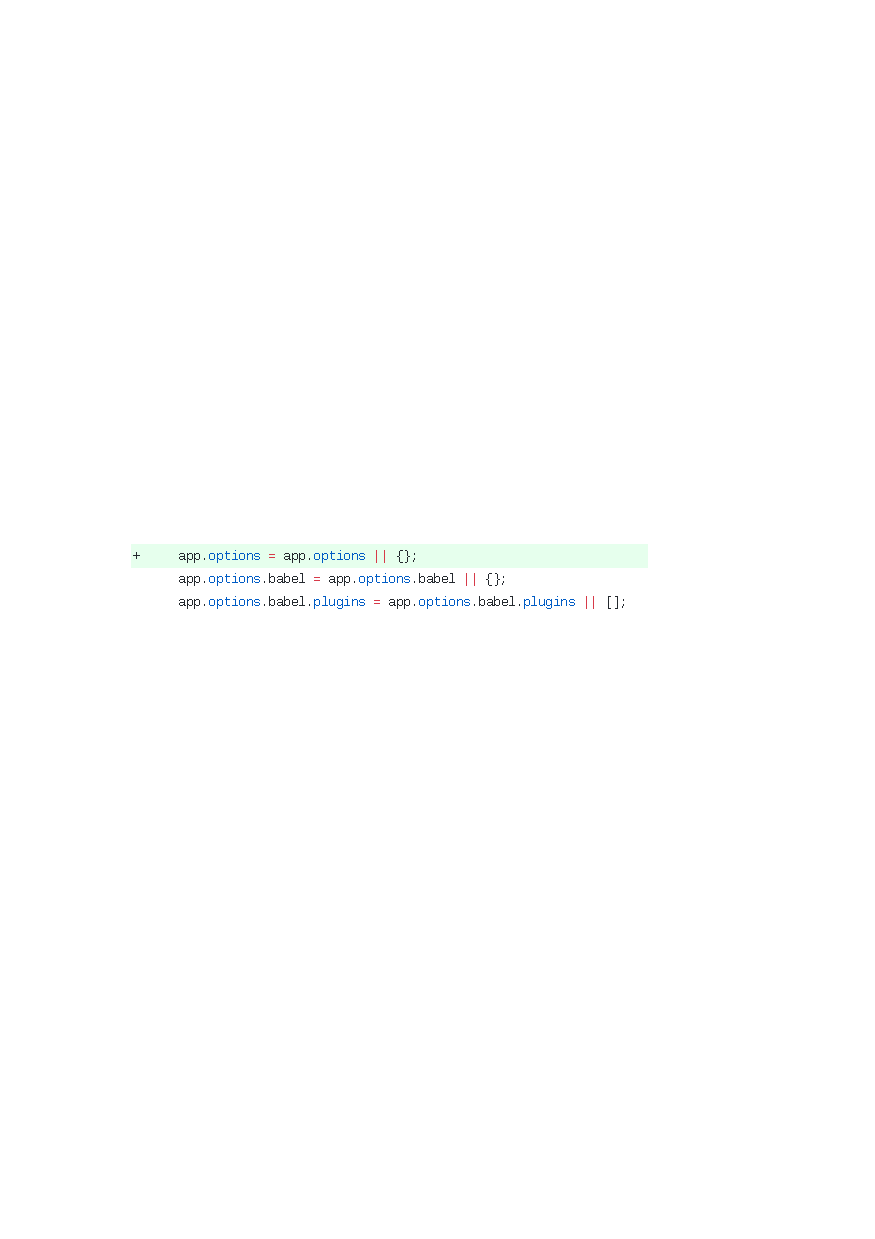
\includegraphics{figuras/bc_category_undefined_object.pdf}
        \caption{Correção do erro de objeto indefinido}
        \label{fig:bc_category_undefined_object}
    \end{figure}{}

    \item \textbf{Código errado}: este caso de \textit{breaking change} ocorreu quando o provedor escreveu um código semanticamente incorreto, gerando um erro na sua execução e afetando o cliente. Em linguagens compilada, esse tipo de erro seria facilmente identificado pelo compilador em tempo de compilação. Foi exatamente isso que a dependência front-matter@0.2.0\footnote{https://github.com/jxson/front-matter/commit/f16fc01d88ff7b93f65ebfbdc957fd66cd5a2002\#diff-168726dbe96b3ce427e7fedce31bb0bcL4} fez. Ao alterar o seu código, o desenvolvedor escreveu duas vezes a mesma variável, como pode ser visto na Figura \ref{fig:bc_category_wrong_code}. Assim como os erros do tipo \textit{undefined object}, os erros dessa categoria são facilmente corrigidos.

    \begin{figure}
        \centering
        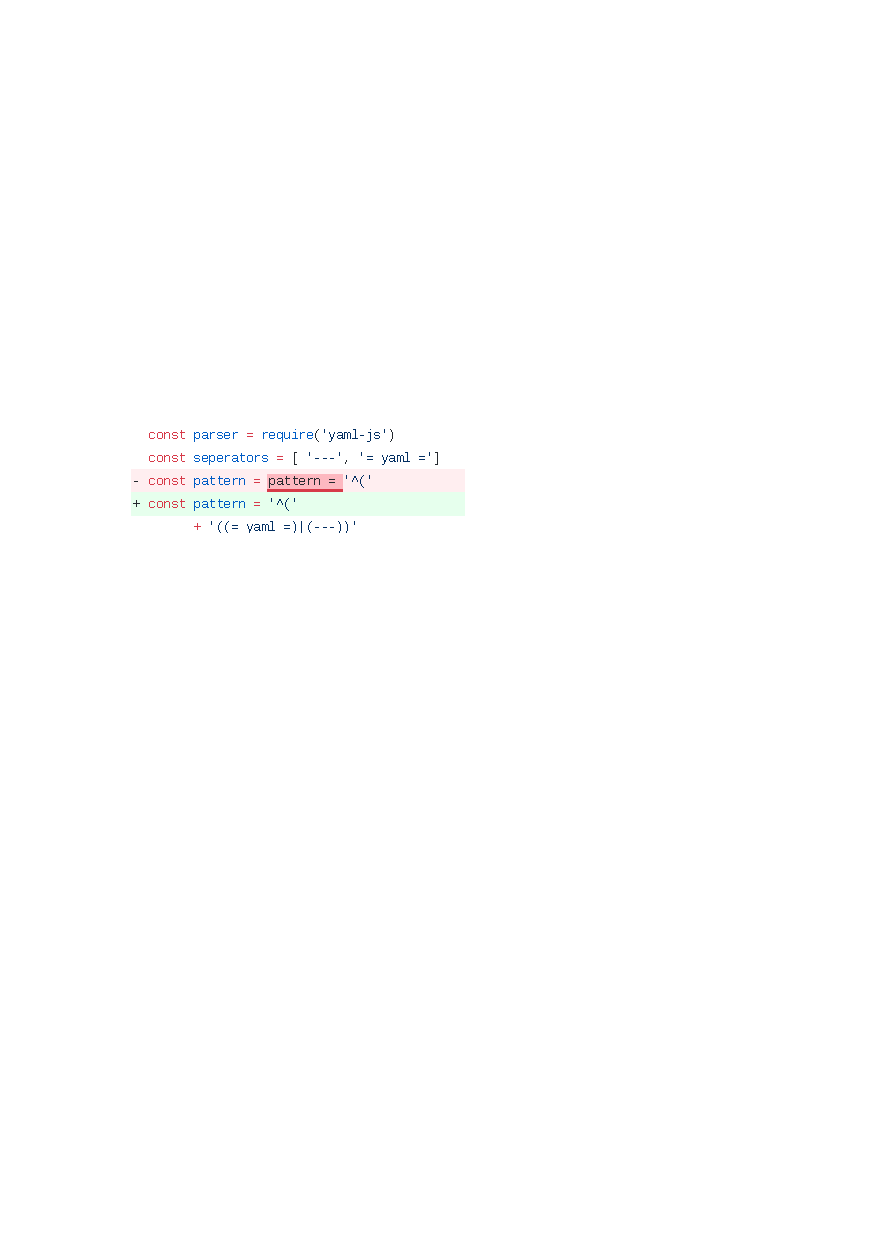
\includegraphics[scale=1.2]{figuras/bc_category_wrong_code.pdf}
        \caption{Código semanticamente incorreto}
        \label{fig:bc_category_wrong_code}
    \end{figure}{}

    \item \textbf{Renomeação de função}: as \textit{breaking changes} relacionadas à esta categoria foram facilmente detectáveis. Quando a mensagem de erro do \textit{node.js} era exibida como \textit{TypeError: var is not a function}, com pouca investigação já era possível saber que uma determinada função não estava mais disponível, ou seja, havia sido removida ou renomeada. E foi exatamente esta \textit{breaking change} que o provedor redis@2.6.0-1\footnote{https://github.com/NodeRedis/node_redis/commit/861749f4d6be28ee861096765e7176dc988024f6\#diff-168726dbe96b3ce427e7fedce31bb0bcL763} introduziu, conforme a \ref{fig:bc_category_renamed_function}.

    \begin{figure}
        \centering
        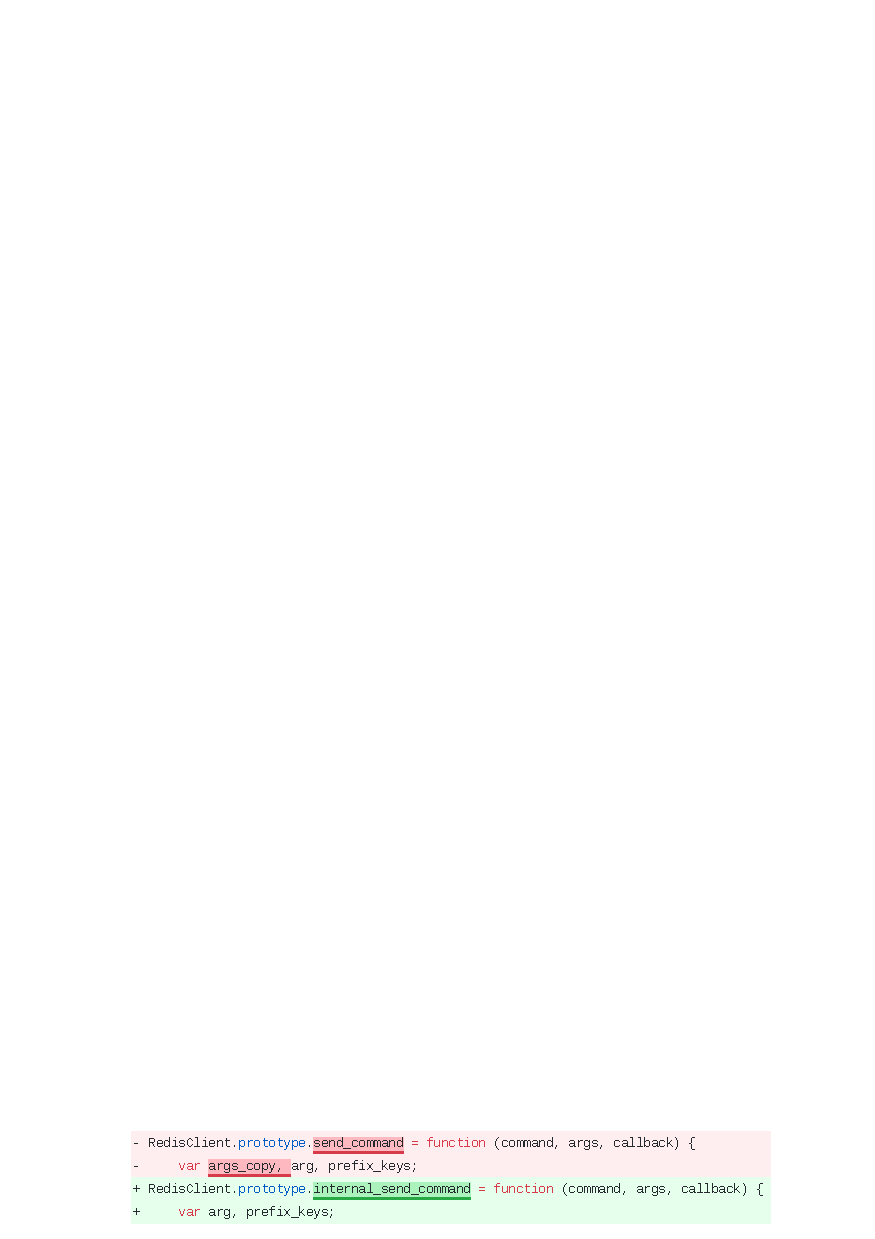
\includegraphics{figuras/bc_category_renamed_function.pdf}
        \caption{Alteração do nome de função}
        \label{fig:bc_category_renamed_function}
    \end{figure}{}

    \item \textbf{Arquivo não encontrado}: os casos de \textit{breaking change} relacionados à esta categoria são aqueles no qual o desenvolvedor realiza um acesso a um arquivo, mas esse não existe. O arquivo requerido pode não existir ou não estar disponível, uma vez que, referenciado no arquivo \textit{.npmignore} -- arquivo utilizado pelo \textit{npm} para ignorar arquivos durante o processo de publicação --, o arquivo existe mas não está disponível, mas também o arquivo pode não existir. Entretanto, o único caso de arquivo não encontrado ocorreu pois o arquivo \textit{index.js} estava indisponível. O provedor \textit{esprima-extract-comments}\footnote{https://www.npmjs.com/package/esprima-extract-comments} utilizava como provedor um \textit{fork} do pacote \textit{esprima}\footnote{https://github.com/ariya/esprima/} e o referenciava em seu  \textit{package.json} para ser descarregado diretamente do \textit{Github}\footnote{https://github.com/jonschlinkert/esprima-extract-comments/blob/6b65a0f52f85bc6fa830d44e352ec3da9e9ef620/package.json\#L47}. Entretanto, o \textit{index.js} desse \textit{fork}, foi referenciado no \textit{.gitignore} e não estava disponível quando o \textit{npm} descarregou o pacote diretamente do \textit{Github}, mas o arquivo estava disponível se esse clone do pacote \textit{esprima} fosse descarregado diretamente do \textit{npm}.

\end{itemize}{}

\subsubsection{Níveis do Versionamento Semântico nos quais as \textit{breaking changes} são introduzidas}
O Versionamento Semântico foi desenvolvido para padronizar o versionamento de \textit{softwares} e facilitar para o cliente decidir quais as novas atualizações que ele deseja receber de um provedor. Entretanto, por vezes os desenvolvedores realizam o versionamento erroneamente, o que pode impactar os clientes negativamente, principalmente quando há \textit{breaking changes} em \textit{releases não-major}. Foi exatamente isso que ocorreu. Dos 45 casos de \textit{breaking changes}, 26 casos foram introduzidos no nível \textit{minor}; 16 casos, \textit{patch}; 2 casos, \textit{major}; e 1 caso foi introduzido em uma \textit{pre-release}, como pode ser visto na Tabela \ref{tab:semver_levels}. Os casos de \textit{breaking changes} que foram introduzidos em \textit{releases major} ou \textit{pre-releases} são \textit{breaking changes} devidamente introduzidas, mas um provedor direto não tratou essas \textit{breaking changes} introduzidas por um provedor indireto, o que acarretou na manifestação da \textit{breaking change} no cliente.

\begin{table}[]
\centering
\begin{tabular}{lr}
\toprule
\textbf{Níveis}      & \textbf{\%} \\ \hline
\textit{Major}       & 4.44\%      \\
\textit{Minor}       & 57.78\%     \\
\textit{Patch}       & 35.56\%     \\
\textit{Pré-release} & 2.22\%      \\ \bottomrule
\end{tabular}
\caption{Porcentagem de \textit{breaking changes} em cada um dos níveis do Versionamento Semântico}
\label{tab:semver_levels}
\end{table}

Mais da metade das \textit{breaking changes} foram introduzidas em \textit{releases minor} (57.78\%). Isso significa que, de acordo com as regras do Versionamento Semântico, os provedores tinham o interesse de publicar novas funcionalidades que mantivessem a compatibilidade com as \textit{releases} anteriores, mas essas novas funcionalidades resultaram em erros nos clientes. Entretanto, essas novas funcionalidades introduzidas pelos provedores podem caracterizar realmente casos de \textit{breaking changes}, no qual os provedores precisaram consertar o código, mas também podem ser apenas novas funcionalidades na qual os clientes precisaram se adequar, pois as \textit{breaking changes} foram causadas não por um erro nos provedores, mas sim por um erro de utilização nos clientes.
\daniel{Será que é viável retomar o exemplo a seguir?}
Foi exatamente isso que ocorreu no exemplo da Figura \ref{fig:bc_category_change_rule_1} em Categorias de \textit{Breaking Changes} na Seção \ref{sec:qp2:results}, na categoria \textit{Alterações de regras}, na qual é possível ver que o provedor desenvolveu uma nova funcionalidade que não continha um erro, mas acabou introduzindo uma \textit{breaking change} no cliente, e essa \textit{breaking change} não foi corrigida pelo provedor, uma vez que essa alteração apenas refletia uma evolução do provedor. Assim sendo, para o cliente o código se trata de uma \textit{breaking change}, mas para o provedor, não.

Para verificar se as \textit{breaking changes} introduzidas em \textit{releases minor} refletem em \textit{breaking changes} no qual os provedores consertaram seu código, ou se refletem em uma nova funcionalidade que os clientes tiveram que se adequar, foi analisado para cada caso de \textit{breaking change} introduzida em \textit{releases minor}, qual pacote que consertou a \textit{breaking change} -- cliente ou provedor -- e qual foi o nível do Versionamento Semântico na qual a \textit{release} que contém a correção foi publicada. Esses dados estão na Figura \ref{fig:semver_fixed}, na qual, dos 26 casos de \textit{breaking changes} introduzidas em \textit{releases minor}, 4 casos foram consertados pelos provedores; 20 pelos clientes; e 2 casos não foram consertados por ambos.

\begin{figure}
    \centering
    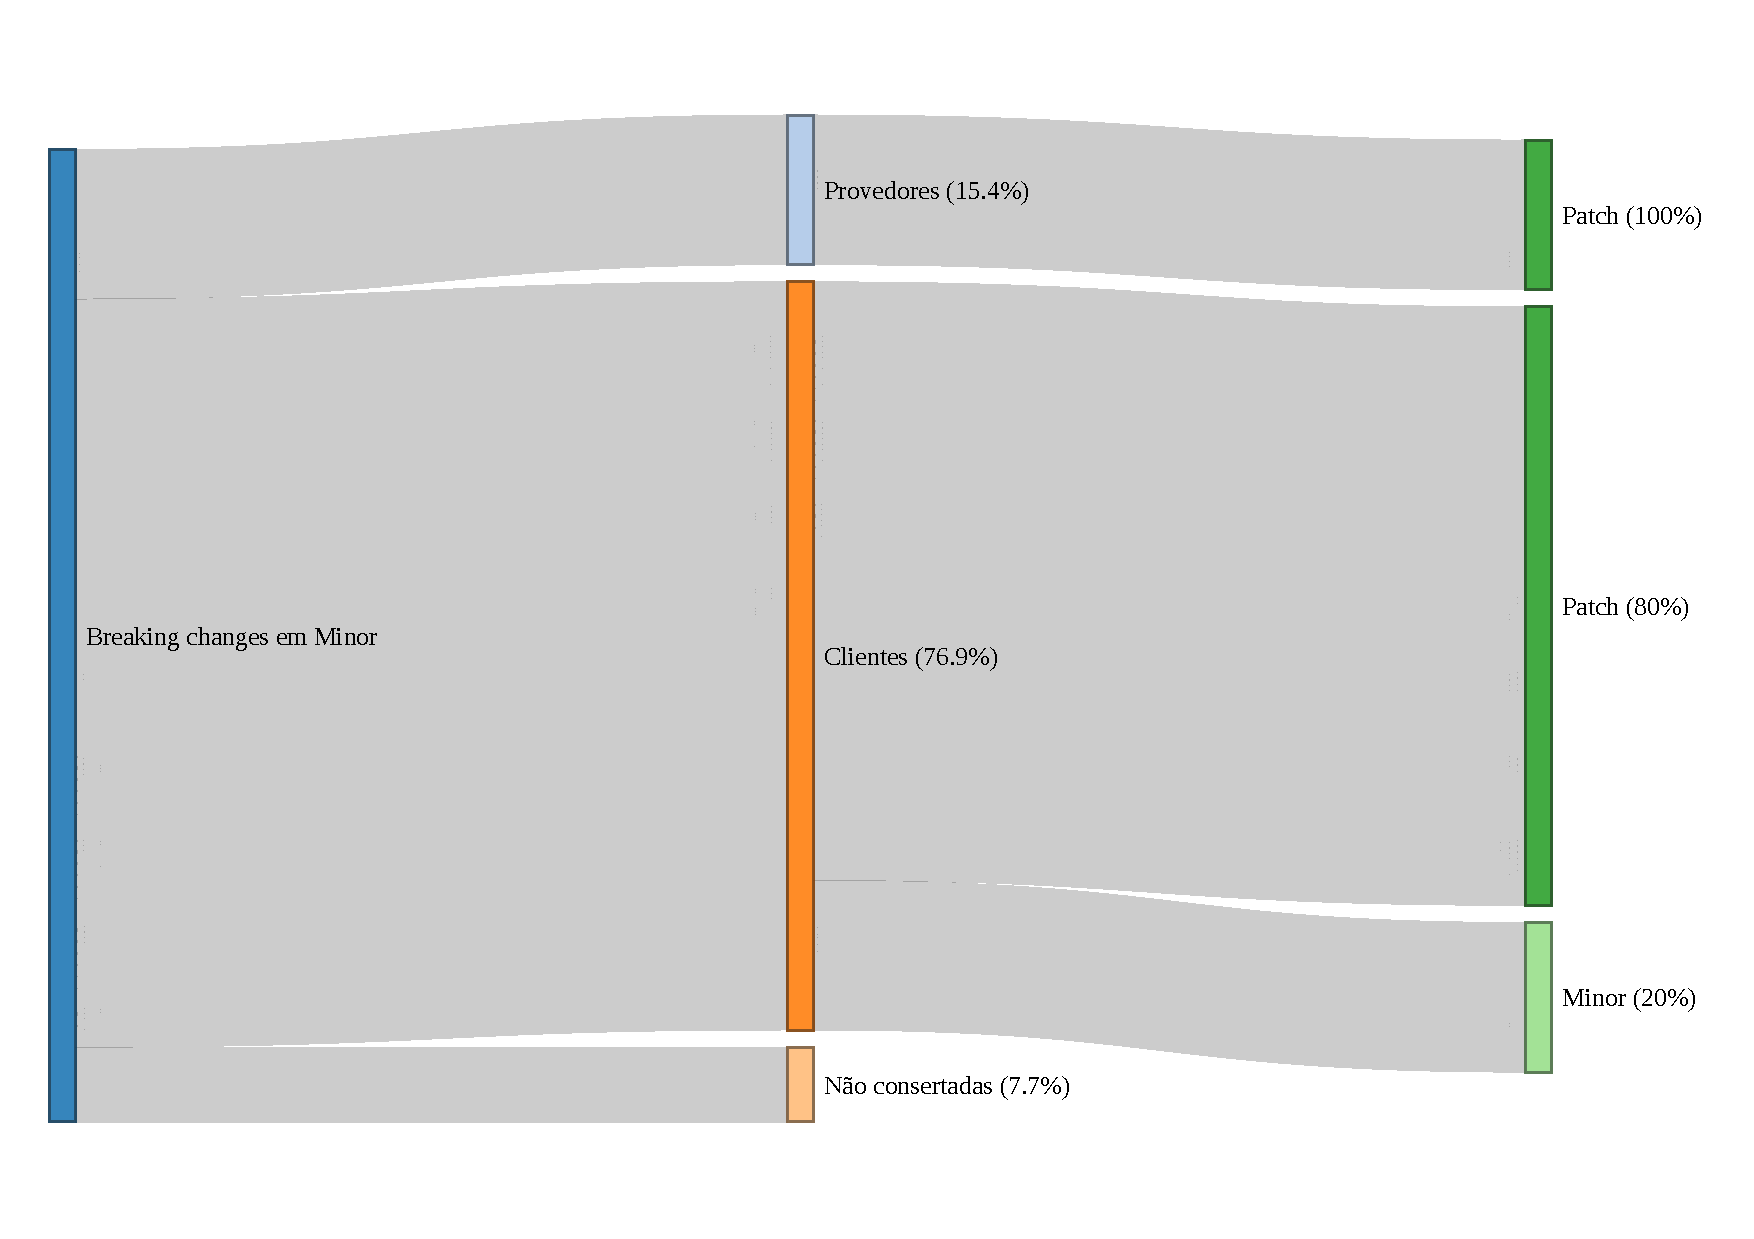
\includegraphics[scale=0.5]{figuras/semver_fixed.pdf}
    \caption{\textit{Breaking changes} consertadas pelo provedor e pelo cliente e os níveis do Versionamento Semântico das \textit{releases} com a correção}
    \label{fig:semver_fixed}
\end{figure}{}

Na Figura \ref{fig:semver_fixed}, é possível verificar que mais da metade dos casos de \textit{breaking changes} que foram introduzidas em \textit{releases minor} (76.9\%) foram consertados pelos clientes. Isso significa que os provedores introduziram novas funcionalidades, que não refletiam em um erro, mas que causaram um comportamento inesperado nos clientes, e foram os clientes os responsáveis por consertar seus códigos para que a nova \textit{release} dos provedores, mesmo sendo retro-compatível, pudesse executar com sucesso. Assim, a maior parte das \textit{breaking changes} não ocorreram porque os provedores introduz um erro em seus códigos e esse erro é cascateado para os clientes, mas sim porque os clientes utilizam o provedor de maneira errada e necessitam consertar o seu código para se adequar às novas funcionalidades introduzidas pelos provedores. Isso é perceptível, pois quando os cliente consertam os seus códigos e os publicam, em 80\% dos casos são publicados em uma \textit{release patch}, ou seja, de acordo com as regras do Versionamento Semântico, os clientes estão consertando algum determinado erro, que pode ser o modo como os clientes utilizam os provedores.

Quando os provedores consertam as \textit{breaking changes}, em 100\% dos casos essa correção é publicada em uma \textit{release patch}, que de acordo com as regras do Versionamento Semântico, são alterações no código que os provedores tinha a intenção de consertar algum determinado erro. Assim, pode-se afirmar que todos os 15.4\% dos casos de \textit{breaking changes} em \textit{releases minor} são realmente \textit{breaking changes} que deveriam ter sido publicadas em \textit{releases major}, mas que por algum motivo, os provedores introduziram em \textit{releases minor} e os clientes foram impactados por essas \textit{breaking changes}.

\subsubsection{Relação entre as categorias das \textit{breaking changes} com os níveis do Versionamento Semântico nos quais foram introduzidas}


Quando o provedor não sabe em qual nível do Versionamento Semântico uma determinada alteração deve ser introduzida, ou quando uma \textit{breaking change} é introduzida acidentalmente, o cliente pode ser impactado pela \textit{breaking change} introduzida  errôneamente em qualquer um dos níveis \textit{minor} ou \textit{patch} do Versionamento Semântico. No geral, as \textit{breaking changes} de uma determinada categoria seguem um padrão de versionamento. A Figura \ref{fig:semver_types} apresenta os casos de \textit{breaking changes} por categoria que foram inseridas em cada um dos níveis do Versionamento Semântico, sendo que os dados de cada categoria foram normalizados. \daniel{foi normalizado para ficar em porcentagem}

\begin{figure}[!h]
	\centering
	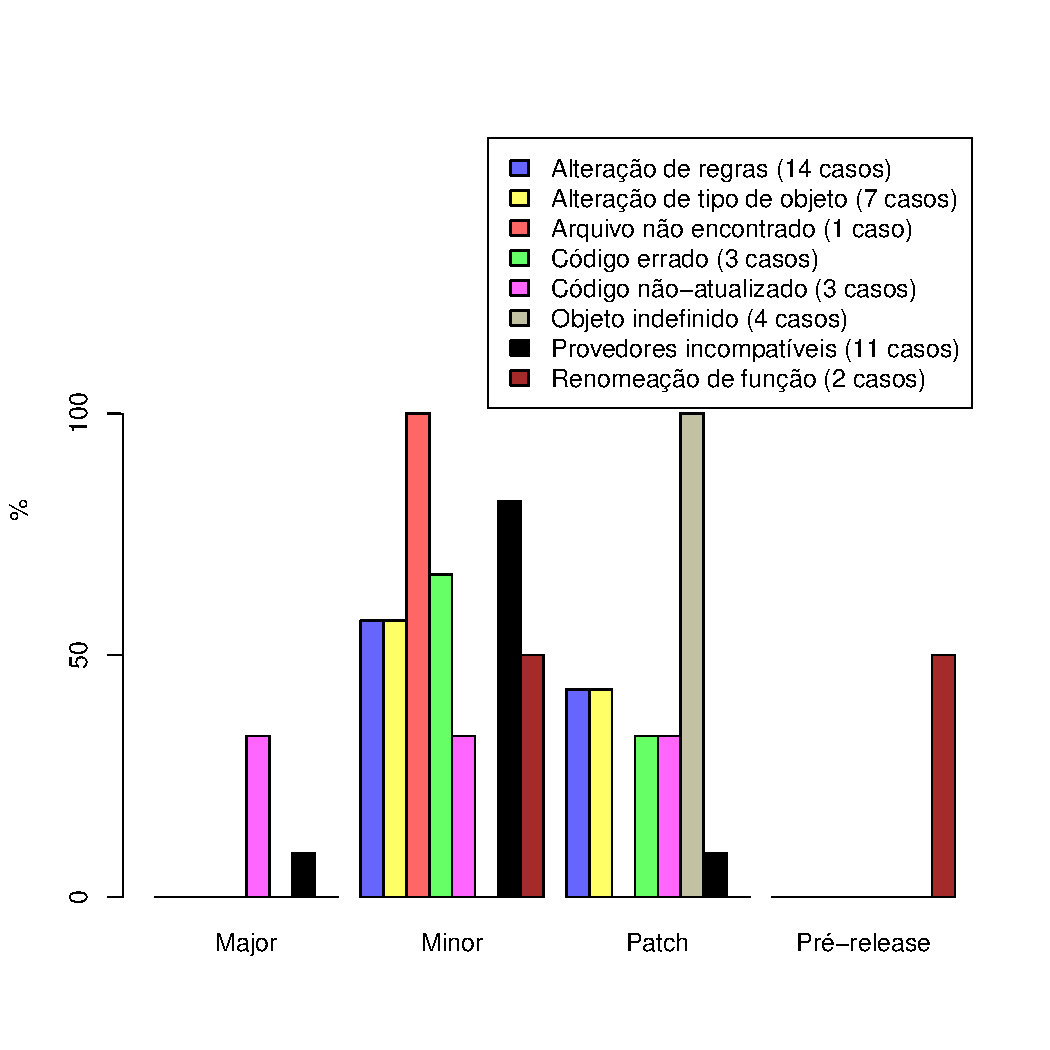
\includegraphics[scale=0.65]{figuras/semver_types.pdf}
	\caption{Os níveis do Versionamento Semântico nos quais as categorias de \textit{breaking changes} foram introduzidas}
	\label{fig:semver_types}
\end{figure}{}

As \textit{breaking changes} introduzidas nos níveis \textit{major} e \textit{pre-release} são \textit{breaking changes} que foram devidamente introduzidas por um provedor indireto, mas um provedor direto aceitou essas \textit{breaking changes}, através de seu \textit{range semver}, e  não alterou o seu código para se adaptar com as \textit{breaking changes}, fazendo com que os clientes fossem impactados por essas \textit{breaking changes}. E as \textit{breaking changes} introduzidas no nível \textit{major} são das categorias \textit{Código não-atualizado} e \textit{Provedores incompatíveis}, que são duas categorias nas quais envolve um provedor direto e um indireto. Ainda sobre essas duas categorias, há casos de \textit{breaking changes} que foram introduzidas tanto em \textit{releases minor} quando em \textit{patch} e, predominantemente,  as \textit{breaking changes} da categoria \textit{Provedores incompatíveis} foram introduzidas em \textit{releases Minor}, ou seja, dois provedores  podem se tornar incompatíveis entre sí após um deles introduzir alterações retro-compatíveis, mas que impacte o outro provedor, fazendo com que o cliente seja impactado por uma \textit{breaking change}.

Duas categorias que tiveram a mesma porcentagem foram a \textit{Alteração de regras} e a \textit{Alteração de tipo de objeto}, que tiveram 60\% e 40\% de seus casos introduzidos em níveis \textit{minor} e \textit{patch}, respectivamente. Os provedores dessas duas categorias introduziram algumas alterações/melhorias em seus códigos que impactaram os clientes com \textit{breaking changes}. Por serem majoritariamente introduzidas em \textit{releases minor}, os provedores tinha a intenção de implementar novas funcionalidades retro-compatíveis ou melhorar as funcionalidades existentes, mas alteraram as funcionalidades que os clientes previamente utilizavam, assim introduzindo uma \textit{breaking change}. Dessa maneira, alguns alterações em funcionalidades já existentes com a intenção de melhora-las deveriam ter sido introduzidas em \textit{releases major}, uma vez que ao invés de melhorar as funcionalidades, os provedores alteraram essas funcionalidades, mostrando que por vezes algumas alterações tornam-se difíceis de serem identificadas, por parte do desenvolvedor, em qual nível do Versionamento Semântico elas devem ser introduzidas.

\section{RQ3. Como os pacotes clientes se recuperam das \textit{breaking changes}?}


\subsubsection{Os clientes que se recuperaram das \textit{breaking changes}}
Quando um provedor introduz uma \textit{breaking change}, o cliente tem três opções para se recuperar: alterar o seu código para que execute mesmo com a \textit{breaking change}; aguardar o provedor corrigir o erro e, logo após, uma pratica comum é alterar a versão aceita do provedor no \textit{package.json}; ou regredir a versão do provedor no \textit{package.json} para utilizar uma que não contenha \textit{breaking changes}. Entretanto, a questão é que, por vezes, os clientes realmente se recuperam das \textit{breaking changes} sem a intervenção dos provedores. Do total de 45 casos de \textit{breaking changes} 30 dos casos foram corrigidos pelos clientes contra 12 dos casos que foram corrigidos pelos provedores  e 3 casos não foram corrigidos por ambos.

A Tabela \ref{tab:fix} apresenta a porcentagem das correções das \textit{breaking changes} pelos provedores e pelos clientes e a mediana do tempo gasto por cada um para que as \textit{breaking changes} fossem corrigidas. Os dias que os provedores gastam para corrigir as \textit{breaking changes} são maiores do que os gastos pelos clientes, uma vez que o provedor precisa ser alertado pelos clientes, análisar o caso, alterar o código, revisar as alterações e publicá-las. E muitas vezes, quando já está sendo preparada uma nova \textit{release}, os provedores podem corrigir a \textit{breaking change} mas publicá-las somente quando a proxima \textit{release} estiver pronta. Em contra partida, os clientes não precisam de todas essas etapas para se recuperar de uma \textit{breaking change}, uma vez que, eles podem simplesmente retroceder a versão do provedor no \textit{package.json} para uma em que não há \textit{breaking changes} e esperar que o mesmo publique uma \textit{release} com a correção. De todos os 30 casos de \textit{breaking changes} nos quais os clientes que corrigiram, em 20 casos foi alterada a versão do provedor no \textit{package.json} para uma versão anterior na qual não havia \textit{breaking changes} -- foi realizado um \textit{downgraded} na versão do provedor --, e a mediana do tempo gasto para os clientes corrigirem a \textit{breaking change} com a alteração da versão do provedor é, também, de 4 dias. Entretanto, mesmo alguns casos no qual o provedor corrigiu o erro, ainda em dois casos os clientes realizaram o \textit{downgraded} do provedor.

\begin{table}[!h]
\centering
	\begin{tabular}{|l|l|l|l|}
		\hline
		\centering
		& Provedor    & Cliente     & Não corrigido                             \\ \hline
		Corrigiu           & 12 (26.7\%) & 30 (66.7\%) & 3 (6.6\%)    \\ \hline
		\textit{Dowgraded} & 2  (4.4\%)  & 20 (44.4\%) & -            \\ \hline
		Dias (mediana)     & 35          & 4           & -            \\ \hline
	\end{tabular}
	\caption{Pacote que corrigiu a \textit{breaking change}, os \textit{downgrade} e a mediana do tempo gasto para ser corrigida}
	\label{tab:fix}
\end{table}
 % Esse capítulo e nome é apenas uma sugestão.
\chapter{Cronograma de Atividades}
\label{cap:cronograma}

Nesta seção são apresentadas as atividades a serem desenvolvidas para a execução da proposta. O cronograma de realização das tarefas é apresentado na Tabela~\ref{tab:cronograma}.

\begin{enumerate}
\item \textbf{Documentação da Ferramenta \textit{BCDetect}}
    \begin{enumerate}
        \item Traduzir a documentação da \textit{BCDetect} para o inglês.
    \end{enumerate}{}
\item \textbf{Análise dos dados da RQ3.}
    \begin{itemize}
        \item Agrupar as ações dos clientes para se recuperarem das \textit{breaking changes}; e
        \item Analisar o tempo que as \textit{breaking changes} levaram para serem consertadas.
    \end{itemize}{}
\item \textbf{Análise dos Resultados.}
    \begin{itemize}
        \item Completar os resultados da QP1; e
        \item Completar os resultados da QP2.
    \end{itemize}{}
\item \textbf{Escrita do TCC 2.}
\item \textbf{Entrega do TCC 2.}
\item \textbf{Apresentação do TCC 2.}
\end{enumerate}

\begin{table}[h!]
\centering
\renewcommand{\arraystretch}{1.3}
\caption{Cronograma de atividades}
\label{tab:cronograma}
\scalefont{0.9}
\begin{tabular}{|c|c|c|c|c|c|}
\hline
\multirow{2}{*}{\textbf{Atividade}} & \multicolumn{2}{l|}{\textbf{2019}} & \multicolumn{3}{l|}{\textbf{2020}} \\ \cline{2-6} 
             & Nov & Dez & Jan & Fev & Mar \\ \hline
\textbf{1}   &  X  &     &     &     &     \\ \hline
\textbf{2}   &  X  &  X  &     &     &     \\ \hline
\textbf{3}   &  X  &  X  &     &     &     \\ \hline
\textbf{4}   &     &  X  &  X  &  X  &     \\ \hline
\textbf{5}   &     &     &     &     &  X  \\ \hline
\textbf{6}   &     &     &     &     &  X  \\ \hline
\end{tabular}
\end{table} % Esse capítulo e nome é apenas uma sugestão.

% Apendices.
%\appendix
%\chapter{Instalação de Ferramentas}
\label{ape:instalacao:ferramentas}

Os apêndices são usados para disponibilizar materiais extras que por questões de espaço ou estilo de escrita não foram colocados diretamente no texto. Por exemplo, \textit{scripts}, instruções de instalação das ferramentas utilizadas pelo trabalho, partes de código fonte e questionários que tenham sido aplicados, tabelas com resultados...

(ATENÇÃO - veja com o seu orientador se é necessário disponibilizar algum material extra sobre algum capítulo em anexo!)



%bibliografia
\bibliographystyle{abntex2-alf}
\bibliography{main} % geração automática das referências a partir do arquivo main.bib

\backmatter
\end{document}
